\documentclass[12pt,letterpaper]{report}

\marginparsep 0pt
\textwidth 6in
\topmargin 0pt
\headsep .5in
\textheight 9.2in
\voffset = 0pt
\hoffset = 0pt
\marginparwidth = 0pt \oddsidemargin = 0pt \sloppy

%Dimensiones de la p�gina
\usepackage[left=2.5cm,top=3cm,right=2.5cm,bottom=2.5cm]{geometry}
%Sangr�a
\setlength{\parindent}{1cm}

%Numeracion
\pagenumbering{arabic}

\usepackage{templateICI}
\usepackage{amsmath,amsfonts}
\usepackage{graphicx}
\usepackage{graphics}
\usepackage[dvips]{epsfig}
\usepackage{times}
\usepackage[latin1]{inputenc}
\usepackage[dvips]{graphicx}
\usepackage[usenames]{color}
\usepackage[spanish]{babel}
\newcommand{\ie}{i.e.}
\newcommand {\out}[1]{}
\newtheorem{definicion}{Definicion}
\usepackage{rotating}
\usepackage{multirow}
\usepackage{array}
\usepackage{longtable}
\usepackage[]{fontenc}
\usepackage{hyperref}

\renewcommand{\shorthandsspanish}{}

\addto\captionsspanish{
\def\listtablename{�ndice de tablas}
\def\tablename{Tabla}}

\sloppy

\begin{document}
	\title{\textbf{Desarrollo de una aplicaci�n m�vil que permita potenciar el desarrollo del lenguaje, en ni�os entre 3 a 6 a�os con trastorno espec�fico en el lenguaje (TEL)}}
	\author{\textbf{Ian Franco Quiroga Far�as}}
	\principaladviser{Carlos Becerra Castro}
	\coprincipaladviser{}
	\firstreader{}
	
	\beforepreface
	\prefacesection{Resumen}
	
	La integraci�n de TICs en el �rea de la educaci�n, permite generar recursos interactivos para el aprendizaje, entregando materiales did�cticos que ense�en y motiven el desarrollo psicomotor y cognitivo de cada persona.
	
	Dentro del �rea de educaci�n, encontramos las escuelas de lenguajes, que se encargan de reforzar, ayudar y ense�ar a ni�os entre 3 a 6 a�os, con dificultades en la expresi�n y comprensi�n en el lenguaje. Estos ni�os, presentan un grado de trastorno espec�fico del lenguaje (TEL).
	
	La falta de innovaci�n e integraci�n TICs en las escuelas de lenguajes, impiden las ense�anzas din�micas de las actividades que actualmente se realizan en papel. 
	Si bien existen aplicaciones m�viles que realicen actividades para los ni�os, la gran mayor�a no reflejan la realidad chilena ni estan enfocados a ni�os con TEL.
	
	Es por ello, tomando los beneficios de usar las TICs en la educaci�n, se propone crear una aplicaci�n m�vil que permita realizar distintas actividades, ense�ando y reforzando los niveles fonol�gico, sem�ntico y morfosint�ctico del lenguaje.
\afterpreface

\listoffigures
\listoftables
%Aqui deben incluir el fuente de cada capitulo, sin su encabezado.



\chapter{Introducci�n}
\label{intr}

En Chile, una de las grandes misiones que tiene el sistema educativo, es fomentar el desarrollo de la educaci�n en todos sus niveles, promoviendo el progreso integral de todas las personas, focalizado a generar igualdad de oportunidades y a la entrega del aprendizaje de calidad para todos los ni�os/as, j�venes y adultos durante su vida \cite{REF1}.\\

Uno de los enfoques donde el ministerio de educaci�n se ha preocupado de realizar mejoras, son en las ense�anzas y cambios curricurales en las aulas de pre-kinder y kinder, donde se forman las habilidades y capacidades m�nimas a ni�os de entre 3 a 6 a�os, para el aprendizaje durante su vida escolar y social.

Pero no todos los ni�os han desarrollado las competencias que son requeridas en la educaci�n b�sica, presentando dificultades en la comprensi�n y expresi�n en el lenguaje. Para estos ni�os que presentan estas dificultades y que no pueden ser explicados por: p�rdida auditiva, da�o cerebral, d�ficit intelectual o motor, factores socioambientales o emocionales, son clasificados como Trastorno Espec�fico del Lenguaje (TEL) \cite{REF2}.\\

El Trastorno Espec�fico del Lenguaje (TEL), es un trastorno grave y duradero que afecta a la adquisici�n del lenguaje desde sus inicios, prolong�ndose durante la infancia y la adolescencia, pudiendo dejar en algunos casos secuelas significativas en la edad adulta.

No todos los ni�os presentan los mismos s�ntomas y con la misma intensidad, en la comprensi�n, en la pronunciaci�n, el uso de la sintaxis o en la capacidad de uso social del lenguaje y de la comunicaci�n, por lo que se debe realizar actividades que abarquen el reforzamiento de las debilidades de cada ni�o \cite{REF3}.\\

Es por ello, que la falta de integraci�n de TICs en el desarrollo del lenguaje, imposibilitan que los ni�os estimulen sus sentidos, potenciando la capacidad de recepci�n y retenci�n de informaci�n a trav�s de recursos interactivos, que ense�en y refuercen el desarrollo psicomotor y el desarrollo cognitivo de cada ni�o. 
Si consideramos que diversos estudios indican que se recuerda el 10\% de lo que se ve, el 20\% de lo que se oye, el 50\%, de lo que se ve y oye, y un 80\% de lo que se ve, oye y hace, la TICs cumplen un papel fundamental para la retenci�n de informaci�n hacia el aprendizaje del ni�o, acercando  as� un poco al mundo digital que se vive hoy en d�a \cite{REF4}.\\

Si bien existen softwares pensados a ni�os que tengan transtorno espec�ficos lenguaje, estas no reflejan la realidad chilena, sobre todo en el mundo de las aplicaciones m�viles.\\

En este trabajo de t�tulo veremos en el \textbf{Capitulo 2} el marco referencial, donde analizaremos el marco conceptual para el domino utilizado en el trabajo. Tambi�n analizaremos el estado de arte, comparando las herramientas que abordan los problemas planteados.\\

En el \textbf{Cap�tulo 3} veremos la definici�n del problema, la forma en que se llevan acabo las actividades seg�n el sistema actual y la naturaleza del cambio de ello.
Adem�s se presenta la metodolog�a de trabajo, la soluci�n a implementar, cumpliendo el objetivo general y los objetivos espec�ficos.
Tambi�n se incluye los requerimientos funcionales y no funcionales, con el diagrama conceptual, diagrama de caso de uso, espec�ficando para cada caso de uso, su caso de uso expandido, diagrama de secuencia y el diagrama de estado, mostrando el  comportamiento general del sistema a desarrollar. \\


En el \textbf{Cap�tulo 4} veremos el dise�o de la aplicaci�n, donde se analizar�n todos los diagramas que representan el sistema, incluyendo el dise�o arquitect�nico donde se explicar� la arquitectura a utilizar en el sistema, el dise�o de la interfaz, representando los casos de usos establecidos en la etapa de an�lisis.\\
Tambi�n se establece el dise�o l�gico, encontrando el diagrama de clases, de despliegue y el de componente y por �ltimo el dise�o de datos y de pruebas, donde se establecer�n los testing a aplicar despu�s de la implementaci�n del sistema.\\


A continuaci�n en el \textbf{Cap�tulo 5}, se presenta la implementaci�n del trabajo de t�tulo, que incluye las herramientas utilizadas para desarrollar el software, el hardware de desarrollo utilizado, el lenguaje de programaci�n y el framework elegido, mostrando las pantallas de interfaz del sistema implementado.\\


En el \textbf{Cap�tulo 6} se incluye la conclusi�n del trabajo de t�tulo.



\chapter{Marco Referencial}
\label{marco}
Dentro el Marco Referencial analizaremos el marco conceptual necesario para comprender el dominio del trabajo de t�tulo utilizado, como tambien as�, analizar las t�cnicas y herramientas existentes que se relacionan al problema planteado.

\section{Marco conceptual}

En el marco conceptual veremos los conceptos necesarios para entender el dominio del trabajo de t�tulo, como tambi�n comparar las herramientas existentes que abarcan a la problem�tica de transtorno espec�fico del lenguaje. 

\subsection{Definici�n del �rea del problema} \label{contexto}

\normalsize

A continuaci�n se abordar�n los conceptos y definiciones fundamentales, que se utilizar�n durante el desarollo de este trabajo de t�tulo.


\subsubsection{Trastorno espec�fico del lenguaje (TEL)} \label{TEL}
\vspace{2mm}
\normalsize

Trastorno espec�fico del lenguaje conocido tambi�n como disfasia, es un trastorno grave y duradero que afecta a la adquisici�n del lenguaje desde sus inicio como tambi�n durante el desarrollo del lenguaje. 
Se define como una dificultad del lenguaje que no es causada por alg�n d�ficit en el nivel neurol�gico, sensorial, intelectual o emocional, afectando el desarrollo del vocabulario, la gram�tica y las habilidades comunicativas.

TEL no afecta de forma homog�nea a cada persona detectada, por lo que afecta con diferentes grados de intensidad a cada componente del lenguaje (fonolog�a, morfol�gia y sintaxis (morfosintaxis), sem�ntica y pragm�tica). Puede afectar a la expresi�n del lenguaje como tambi�n a la comprensi�n del lenguaje.

Las dificultades  y habilidades de los ni�os afectados evolucionan a medida que transcurre el tiempo, superando algunos problemas detectados y adquiriendo otros nuevos, que afectan en sus entornos sociales y escolares.

En TEL el problema principal est� enfocado en el lenguaje oral, pero tambi�n presentan problemas en otras �reas del desarrollo. Los ni�os con TEL tienen m�s probabilidad de tener problemas sociales, emocionales, de conducta y problemas significativos para la adquisici�n del aprendizaje del lenguaje \cite{atelga}.


\subsubsection{Niveles del lenguaje} \label{nivelesdelenguaje}


Dentro de los niveles de lenguaje que afecta TEL \cite{conciencia}, podemos encontrar los siguientes:


\begin{itemize}
	
	\item \textbf{Nivel Fonol�gico}: 
	
	El sonido de las letras, palabras y la entonaci�n de cada una de ellas. Los ni�os pueden pueden repetir las s�labas de una palabra pero no la palabra completa, lo mismo para las palabras nuevas. Tambi�n presentando dificultades en articulaciones y modulaciones en palabras largas.
	
	\item \textbf{Nivel Sem�ntico}: 
	
	El significado de las palabras. Los ni�os con TEL presentan un vocabulario restringido, reflejando una evidente dificultad en aprender nuevas palabras, dado que presentan falencias en la construcci�n de las representaciones fonol�gicas duraderas.
	
	Tambi�n presentan problemas de lentitud  en el reconocimiento de palabras,  para denominar palabras  y dificultades en establecer relaciones l�xicas. \\
	
	\item \textbf{Nivel Morfosint�ctico}: 
	
	La categorizaci�n de las palabras, por ejemplo si son verbos, preposiciones, pronombres, entre otros. Tambi�n  sobre la utilizaci�n de estas palabras en la formaci�n y el empleo de las oraciones, que afectan a la complejidad de la sintaxis, llegando ser ininteligible el lenguaje. \\
	
	\item \textbf{Nivel Pragm�tico}: 
	
	El uso del lenguaje var�a seg�n el contexto. 
	
	Por ejemplo, en iniciaciones y mantenimientos de temas de conversaci�n, algunos ni�os no presentan dificultades en adicionar temas nuevos dentro de la conversaci�n, pero a�n as� presentan  problemas en mantener los mismos temas que ellos introducen o temas que los adultos introducen.
	
	En cambio en el discurso, presentan dificultades en mantener la estructura de un discurso, impidiendo la capacidad de responder preguntas literales referidas a un texto, como tambi�n, no aprovechan el recurso lingu�stico de la  narraci�n, exposici�n o conversaci�n.
	
	
	
\end{itemize}

\subsection{Estado del Arte}
\label{tec}
\vspace{1mm}
\normalsize

En esta secci�n veremos las herramientas y t�cnicas encontradas, realizando un an�lisis de cada una ellas y generando una comparaci�n entre ellas.  



\subsubsection{T�cnicas y m�todos existentes}


Dentro de la t�cnicas y m�todos de evaluaci�n para la detecci�n de trastorno de lenguaje en ni�os, en Chile, se aplican 2 test con diferentes metodolog�as para la medici�n de TEL, que son las siguientes:

\subsubsection{TECAL}

Es un test para la comprensi�n auditiva del lenguaje (TECAL) en ni�os entre 3 a 6 a�os 11 meses, que consta de 101 items, donde 
41 items eval�an el vocabulario, 48 items eval�an morfolog�a y 12 items corresponde a sintaxis.

Se aplican de forma individual y consiste que el ni�o escuche un est�mulo auditivo y que asocie ese est�mulo a la l�mina presentada.

Cada l�mina contiene 3 dibujos, 1 dibujo que corresponde a la respuesta correcta, otro de constraste referente y el otro que act�a como distractor, anotando los resultados en una hoja de respuesta.

Cada respuesta correcta corresponde a 1 punto, sumando los puntos de cada secci�n se establece la interpretaci�n \cite{tecal}.

\subsubsection{TEPROSIF}

Es un test que eval�a los procesos de simplificaci�n fonol�gica  en ni�os de 3 a�os  hasta 5 a�os 11 meses.

Consta de 36 items, constituidos cada uno por una palabra. Las palabras tiene la caracter�stica de ser distinta metr�a (mono, bi, tri y polis�labos) con diferentes estructuras (s�laba trabadas, etc.).

El test incluye 36 l�minas en blanco negro la que cada una de ellas se encuentran divididas en dos mitades. En la mitad superior  se respresenta la palabra a evaluar y un objeto que crea el contexto para esa palabra. En la mitad inferior se 	encuentran  ambos dibujos que est�n relacionados.

La modalidad aplicada pertenece a la imitaci�n diferida, al cual permite que exista el tiempo necesario  en la audici�n de la palabra y la producci�n de esa palabra, para que el ni�o exprese su proceso fonol�gico \cite{teprosif}.\\

\vspace{1mm}

\normalsize

\subsubsection{Herramientas existentes}

Dentro de las herramientas relacionadas con el aprendizaje en el lenguaje, encontramos softwares y aplicaciones m�viles que son aplicados a ni�os de rango 3 a 6 a�os. Estas herramientas son las siguientes:



\vspace{2mm}
\subsubsection{Nivel Sem�ntico}

\begin{itemize}
	
	\item \textbf{EXLER:} Desarrollada por la Escuela de Patolog�a del Lenguaje (EPL), Barcelona.\\
	El objetivo principal de este programa es el desarrollo l�xico, enfocado a los ni�os con trastornos espec�ficos del lenguaje.\\
	La metodolog�a utilizada es entregar diferentes campos sem�nticos (la casa, la cocina, el ba�o, el pescador y el pueblo del pescador), realizando para cada uno 5 tipos de actividades: Exploraci�n del nombre, comprensi�n verbal, comprensi�n escrita, dictado y la denominaci�n escrita \cite{exler}.\\
	
	El software de escritorio (Figura \ref{exler}) permite:
	
	\begin{itemize}
		
		\item Desarrollar y ampliar el vocabulario del ni�o.
		\item Estimular la 	atenci�n y la comprensi�n auditiva del ni�o.
		\item Estimular y ejercitar la comprensi�n escrita.
		\item Ejercitar la transcripci�n del lenguaje oral a lenguaje escrito.
		\item Ayudar la correcta escritura de cada palabra.
		
	\end{itemize}
	
	\begin{figure}[htf]
		\begin{center}
			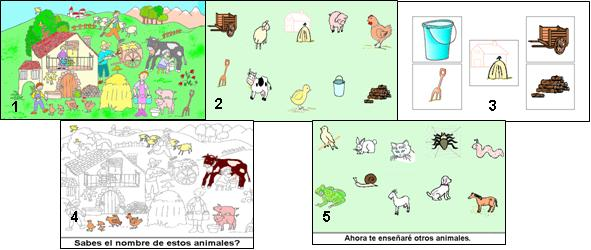
\includegraphics[width=9cm,height=5cm] {imagenes/exler.jpg}
		\end{center}
		\caption{Programa EXLER, EPL} \label{exler}
	\end{figure}
	
	
	\newpage
	\item \textbf{Nociones Espaciales:} Aplicaci�n m�vil creada por la compa��a Fonolab \cite{nociones}, Santiago de Chile.
	
	Nociones Espaciales (Figura \ref{nociones}) es un juego en donde el ni�o deber� arrastrar y ubicar cada elemento en la posici�n en la que corresponda.
	
	El juego cuenta con 12 etapas, y a medida que avanza cada etapa, se aumenta la complejitud del juego.
	
	El juego se encuentra disponible en Android y IOS por un valor de \$ 5 d�lares.
	Usuarios que han comprado e instalado la aplicaci�n: 5.\\
	
	
\end{itemize}


\begin{figure}[htf]
	\begin{center}
		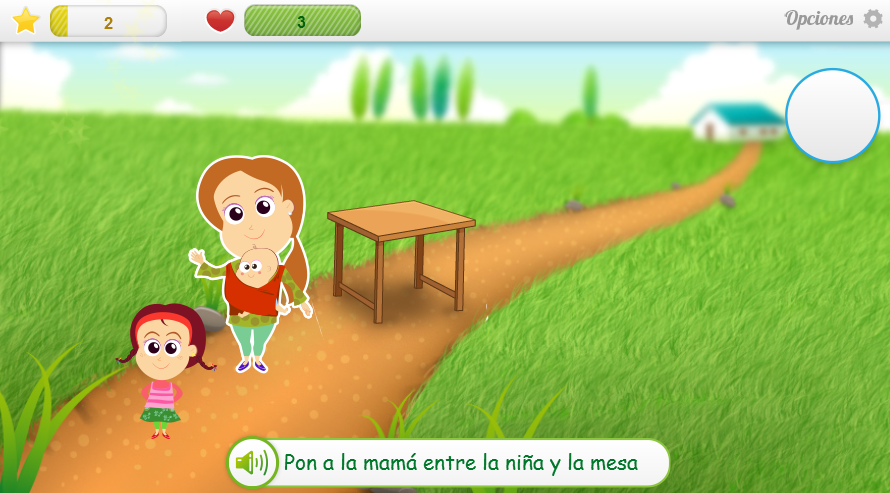
\includegraphics[width=10cm,height=6cm] {imagenes/espaciales.png}
	\end{center}
	\caption{Nociones Espaciales, Fonolab}\label{nociones}
\end{figure}


\vspace{2mm}
\subsubsection{Nivel Morfosint�ctico}

\begin{itemize}
	\item \textbf{ESPIRAL Morfosintaxis:} Software de escritorio desarrollado por Onda Educa \cite{morfo}, Zaragoza.
	
	Esta herramienta (Figura \ref{espiral}) permite trabajar morfemas dependientes y determinantes, morfolog�a verbal, interrogaciones, pronombres, preposiciones y conjugaciones verbales.
	
	El software consta de dos grandes bloques, conteniendo cada bloque 6 etapas que desarrollan distintas actividades, apoyado con im�genes intuitivas, funci�n de ayuda, adem�s de l�minas manipulativas, ense�ando de forma interactiva, apuntando el trabajo individual y al trabajo grupal.
	
	
	\begin{figure}[htf]
		\begin{center}
			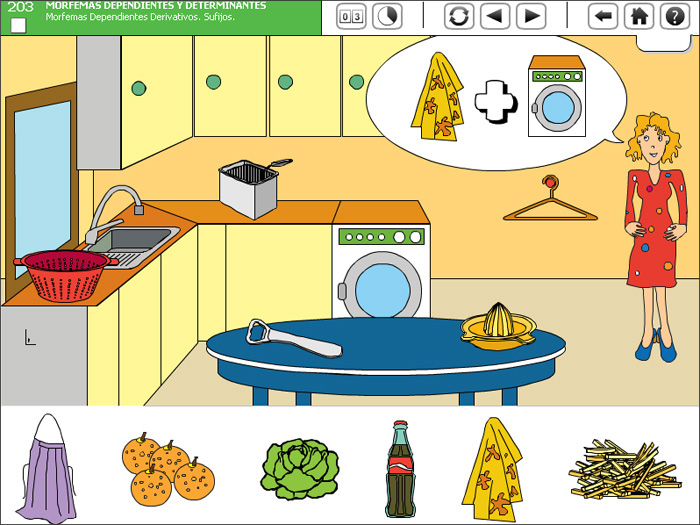
\includegraphics[width=10cm,height=6cm] {imagenes/espiral.jpg}
		\end{center}
		\caption{ESPIRAL Morfosintaxis, Onda Educa}\label{espiral}
	\end{figure}	
	
	\item \textbf{La frase y yo. Estructurando el lenguaje:} Programa creado por Eugenio Corbal�n \cite{recursos}.
	
	Se centra en el nivel morfosint�ctico, permitiendo dentro de sus actividades, el trabajo  de la esructura de frases sencillas S-V-C con apoyo visual, utilizando situaciones de la vida diaria y m�s cercanas a los ni�os (Figura \ref{frase}).\\
	
	\begin{figure}[htf]
		\begin{center}
			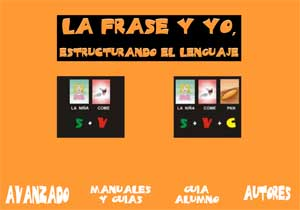
\includegraphics[width=10cm,height=6cm] {imagenes/frase.jpg}
		\end{center}
		\caption{La frase y yo. Estructurando el lenguaje, Eugenio Corbal�n}\label{frase}
	\end{figure}
	
	
	
\end{itemize}

\newpage
\vspace{2mm}
\subsubsection{Nivel Fonol�gico}

\begin{itemize}
	
	\item \textbf{Segmenta S�labas:} Aplicaci�n m�vil creada por la compa��a Fonolab \cite{segmenta}, Santiago de Chile.
	
	Segmenta S�laba (Figura \ref{segfon}) es un juego que tiene por objetivo estimular y potenciar el desarrollo de la conciencia fonol�gica a trav�s de la segmentaci�n y manipulaci�n de s�labas.
	Durante el juego, el ni�o controla un personaje  que deber� ir saltando para "atrapar" las s�labas que corresponde a cada palabra. As� el ni�o aprender� a asociar las s�labas de cada palabra.
	
	El juego se encuentra disponible en Android y IOS por un valor de \$ 2 d�lares.
	Usuarios que han comprado e instalado la aplicaci�n: 5.
	
	\begin{figure}[htf]
		\begin{center}
			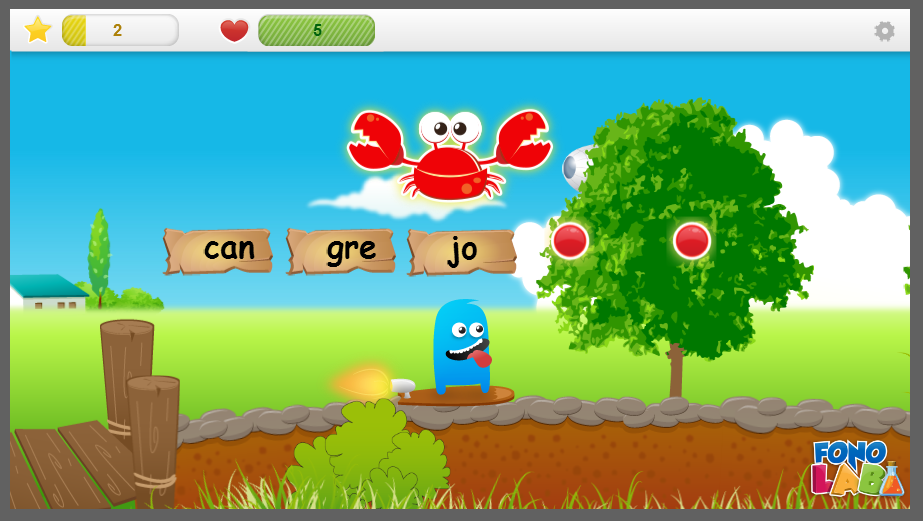
\includegraphics[width=10cm,height=6cm] {imagenes/silabas.png}
		\end{center}
		\caption{Segmenta S�labas, Fonolab} \label{segfon}
	\end{figure}
	
	
	\newpage
	\item \textbf{Proyect@ Logomon}: Aplicaci�n m�vil (Videojuego) creado por Daniel Alonso Hern�ndez Jara, Ingeniero Civil en Inform�tica, Universidad de Valpara�so.
	El videojuego (Figura \ref{log}) que se basa en el uso de pseudopalabras o logotomas, los cuales crean una representaci�n de facciones sonoras, sin sentido ni significado, formadas por consonantes y vocales arbitrarias.
	Para esto se utiliza el reconocimiento de voz para la pronunciaci�n de logotomas, evaluando con pruebas de diagn�sticos \cite{logo}.
	
	\begin{figure}[htf]
		\begin{center}
			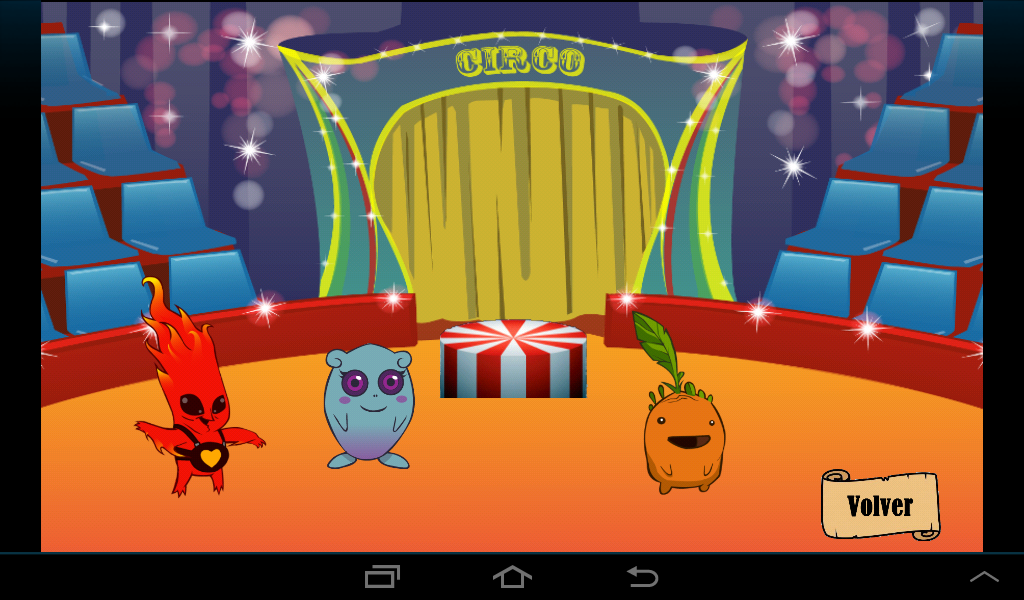
\includegraphics[width=10cm,height=6cm] {imagenes/logomon.png}
		\end{center}
		\caption{Proyect@ Logomon, Universidad de Valpara�so}\label{log}
	\end{figure}
	
	
	
\end{itemize}


\newpage
\vspace{2mm}

\subsection{Comparaci�n entre t�cnicas y herramientas existentes} \label{comp}



Entre las t�cnicas y herramientas investigadas, podemos diferenciar que cada herramienta y test estan enfocadas a cada nivel del lenguaje, por lo que no hay un software que desarrolle la mayor�a de los niveles del lenguaje (Tabla \ref{compherra}).

Dentro de los recursos de cada software, los programas de escritorio presentan l�minas y dibujos  de forma monotoma, en comparaci�n de la forma interactiva que se entrega en las aplicaciones m�viles investigadas.

A pesar que encontramos aplicaciones m�viles que reflejen la realidad chilena enfocadas a TEL, estas son muy escasas y son de pagos, imposibilitando a las personas que no tienen los medios para pagar en una tienda de aplicaciones m�viles.

La gran mayor�a de los software investigados no interact�an con la voz del ni�o, a excepci�n de la herramienta "Proyect@ Logomon" que utiliza el reconocimiento de voz en las actividades del juego.\\
Tomando en consideraci�n lo descrito anteriormente, la aplicaci�n m�vil a desarrollar en el trabajo de t�tulo, innovor� con la inclusi�n de varios niveles del lenguaje, contar con recursos interactivos, adem�s de grabar la voz del ni�o para desarrollar el nivel fonol�gico. 
Adem�s la aplicaci�n m�vil a desarrollar ser� totalmente gratuita.


\begin{table}[htf]
	\begin{center}
		\begin{tabular}{| p{2.7cm} | p{1.7cm}  | p{1.9cm} |p{2.3cm} | p{1.8cm} |p{1.8cm} | p{1.8cm} |}
			\hline
			
			\multicolumn{7}{|c|}{\textbf{\textit{Herramientas existentes}}} \\ \hline \hline
			\textit{\textbf{Caracter�stica}} & 
			\textit{\textbf{EXLER}} &
			\textit{\textbf{Nociones Espaciales}} & 
			\textit{\textbf{Espiral Morfosintaxis}} & 
			\textit{\textbf{La frase y yo}} & 
			\textit{\textbf{Segmenta S�labas}} & 
			\textit{\textbf{Proyect@ Logomon}} \\ \hline \hline
			
			
			Tipo de 
			
			Software& 
			Escritorio& 
			M�vil& 
			Escritorio& 
			Web& 
			M�vil& 
			M�vil\\ \hline
			
			Realidad 
			
			Chilena& 
			No& 
			Si& 
			No& 
			No& 
			Si& 
			Si\\ \hline
			
			Licencia& 
			Pago& 
			Pago& 
			Pago& 
			Gratis& 
			Pago& 
			Gratis\\ \hline
			
			Voz del 
			
			usuario& 
			No& 
			No& 
			No& 
			No& 
			No& 
			Si\\ \hline
			
			Nivel 
			
			Sem�ntico& 
			Si&
			Si&
			No&
			No&
			No&
			No \\ \hline
			
			Nivel
			
			Morfosint�ctico& 
			No&
			No&
			Si&
			Si&
			No&
			No \\ \hline
			
			Nivel
			
			Fonol�gico& 
			No&
			No&
			No&
			No&
			Si&
			Si \\ \hline
			
		\end{tabular}
	\end{center}
	\caption{Comparaci�n de las herramientas investigadas}\label{compherra}
\end{table}

\chapter{Definici�n del Problema y An�lisis}
\label{definicion}

\section{Definici�n del problema} \label{prob}

\vspace{1mm}

\normalsize

La falta de innovaci�n en integrar TICs en las aulas de las escuelas de lenguajes, impiden ense�ar de forma din�mica e interactiva sobre el mejoramiento de las falencias detectadas en los ni�os con trastorno en el lenguaje, considerando que entre 3\% - 10\% de la poblaci�n infantil presenta alg�n tipo de d�ficit en el lenguaje \cite {REF5}.\\

Problemas en la expresi�n y comprensi�n en el lenguaje oral, carencia en las reglas gramaticales,  dificultades en articular los fonemas de una palabra, dificultades para discriminar sonidos (tonos ling��sticos y no ling��sticos), son las falencias que presentan un ni�o detectado con trastorno  en el lenguaje \cite{REF6} .

Si estos problemas no son tratados a tiempo, con llevan al retraso en el aprendizaje durante toda su vida escolar, afectando a su vida social y futuramente su vida laboral.\\

Si bien existen aplicaciones pensado a ni�os desde los 3-6 a�os, no estan enfocados a los peque�os que presentan alg�n grado del  trastorno en el lenguaje, s�lo abarcan un nivel del lenguaje, imposibilitando  mejorar y reforzar las debilidades detectadas en todos los niveles del lenguaje, que pueden ser centrados en una sola aplicaci�n.


\newpage
\vspace{1mm}

\subsection{Sistema actual y naturaleza del cambio}

\vspace{1mm}

\normalsize

Actualmente los sistemas enfocados a potenciar el desarrollo del lenguaje en TEL, se centran en un nivel espec�fico del lenguaje, utilizando im�genes, palabras y audios para las actividades de cada software.\\

Tambi�n el uso de TICs en aulas de educaci�n parvularia es casi nula, dado que no cuentan con computadores y dispositivos m�viles para la utilizaci�n de software que permitan mejorar el lenguaje de los ni�os, adem�s que la gran mayor�a de los software desarrollados, deben ser adqueridos a trav�s de un medio de pago para obtener la licencia del software, limitando m�s a�n el acceso a escuelas, colegios y jardines que carecen el recurso para obtenerlo.\\ 

Por lo mencionado anteriormente, se desarrollar� una aplicaci�n m�vil gratuita, que permita reunir diferentes actividades en un juego para ni�os entre 3 a 6 a�os con trastorno espec�fico del lenguaje, enfocado en los niveles Fonol�gico, Sem�ntico y Morfosint�ctico.
Esto permitir� que cada ni�o utilice otra forma de realizar actividades que actualmente lo realizan en papel, entregando las ense�anzas interactivamente.\\

La aplicaci�n m�vil tendr� la opci�n de seleccionar dos ambientes, en las cuales cada una tendr� tres actividades que es el cuento, las adivinanzas y el pictograma musica, diversificando el contenido en la aplicaci�n. 


\vspace{1mm}
\subsection{Metodolog�a}

La metodolog�a a utilizar durante todo el proyecto ser� esencialmente en cascada (Figura \ref{meto}), a excepci�n de la etapa de desarrollo que ser� de forma incremental, donde se realizar�n pruebas unitarias a medida que las actividades se vayan implementando.\\

En la etapa de an�lisis se investigar� sobre los conceptos involucrados en el trabajo de t�tulo, sobre las herramientas existentes y por �ltimo el levantamiento de requerimientos funcionales y no funcionales que se desarrollar�.\\

Luego en la etapa de dise�o, se obtendran los prototipos preliminares y finales de la interfaz de la aplicaci�n. Adem�s se incluir� la documentaci�n sobre la construcci�n del sistema, a trav�s de diagramas y modelos.\\

En la etapa de desarrollo, la implementaci�n del sistema ser� incremental, encontrando dos ambientes del juego, en donde cada ambiente se desarrollar� 3 actividades. Cada ambiente tendr� testing de desarrollo, donde se realizar�n pruebas unitarias.

\newpage
Por otro lado, una vez finalizada la etapa de desarrollo y testing de desarrollo, se ejecutar� la etapa de testing general, en donde se realizar� una prueba de integraci�n sobre las funcionalidades implementadas y testing con usuarios sobre la usabilidad de la aplicaci�n.\\

Por �ltimo la etapa de implantanci�n, donde se pondr� en la puesta en marcha la aplicaci�n, donde podr� ser utilizada y descargada desde la tienda de android.\\

\begin{figure}[htf]
	\begin{center}
		\includegraphics[width=12cm,height=14cm] {imagenes/metodologia.png}
	\end{center}
	\caption{Metodolog�a utilizada en el trabajo de t�tulo.}\label{meto}
\end{figure}


\clearpage
\newpage
\section{Soluci�n propuesta}

\vspace{1mm}

\normalsize

Desarrollo de una aplicaci�n m�vil gratuita (juego) para dispositivos Tablets de bajo costo (Android), que permita:

\begin{itemize}
	
	\item Seleccionar dos ambientes en el juego, para generar tres actividades, el cuento, las adivinanzas y el pictograma musical, presentando diversos recursos interactivos.
	Ej. Un ambiente tendr� dos cuentos, y para cada cuento, un juego de adivinazas y un juego de pictograma musical.
	
	\item La aplicaci�n tendr� dos personajes principales los cuales podr�n ser elegido por el ni�o. Ej. Un ni�o o una ni�a.
	
	
	\item Creaci�n de un diccionario en las actividades, que permita al ni�o ampliar su vocabulario, incluyendo im�genes y palabras que podr�n incluir sonido de �stas.
	
	
	\item Inclusi�n de sonidos en las diferentes actividades que mejoren la conciencia fonol�gica de cada ni�o, asociando el sonido a las im�genes o a las palabras.
	Ej. Cuando aparece la imagen o palabra del le�n en el diccionario, podr� reproducir el sonido de la palabra le�n o el rugido del le�n.
		

	\item En la actividades de las adivinanzas tendr�n la opci�n de "pistas", que ayudar�n al ni�o a resolver cada pregunta.
	
	\item En la actividades de las pictograma musical tendr�n la opci�n de "reproducir canci�n", que ayudar� al ni�o a reproducir nuevamente la canci�n, permitiendo al ni�o completar m�s facilmente las im�genes correctas en la letra.
	
	\item Grabar las voces del ni�o en las actividades, permitiendo reproducir esa grabaci�n para mejorar el �rea de la fon�tica. 
	Ej. Grabar la voz del ni�o en la actividad pictograma musical, para reproducir en conjunto de una canci�n.
	
	\item Adaptar las actividades que trabajan en el lenguaje, a la realidad chilena.
	
	
\end{itemize}

\newpage
\vspace{1mm}
\subsection{Objetivos}


\vspace{2mm}
\subsubsection{Objetivo General}

Desarrollar una aplicaci�n m�vil  que permita potenciar el aprendizaje del lenguaje, realizando soporte en el nivel de fonol�gico,  el nivel sem�ntico y el nivel morfosint�ctico, en ni�os entre 3-6 a�os, por medio de juegos interactivos.


\vspace{2mm}
\subsubsection{Objetivos Espec�ficos}
\begin{itemize}
	
	\item Generar y desarrollar  distintos ambientes o escenarios, que permitan diversificar el contenido y las actividades dentro de la aplicaci�n. 
	Ej. Una selva, la Ant�rtida. 
	
	\item Establecer y dise�ar las actividades del cuento, adivinanzas y pictograma musical, que estar�n disponible en la aplicaci�n.
	
	\item Integraci�n de un diccionario para ampliar el vocabulario del ni�o.
	
	\item Gestionar capturas de voces, que permitan reforzar la conciencia fonol�gica en los ni�os.
	
	\item Integraci�n de una barra herramienta que permita acceder al diccionario y grabar la voz del ni�o, disponible en las actividades de la aplicaci�n.
	
	\item Dise�ar e incluir una introducci�n que permita explicar la aplicaci�n y sus herramientas.
	
	
\end{itemize}


\clearpage
\newpage
\vspace{1mm}
\subsection{Especificaci�n de requerimientos}

Dentro esta secci�n, se especificar�n los requerimientos del sistema, los tipos de usuario y la documentaci�n de los diagramas que reflejen el sistema a desarrollar durante el trabajo de t�tulo.

\vspace{2mm}
\subsubsection{Requerimientos Funcionales}

Los requerimientos funcionales son todos aquellos que el cliente desea que realice la aplicaci�n o sistema, identificados en la Tabla \ref{reqfun} y Tabla \ref{reqfun2}:

\begin{table}[htf]
	\begin{center}
		\begin{tabular}{| p{2.5cm} | p{8cm}|}
			\hline
			
			\multicolumn{2}{|c|}{\textbf{\textit{Requerimientos Funcionales}}} \\ \hline \hline
			\textit{\textbf{Identificador}} & 
			\textit{\textbf{Requerimiento}} \\ \hline \hline
			
			
			REF001&  
			Creaci�n e incorporaci�n de un micr�fono con la funcionalidad de grabar la voz del ni�o, pudiendo reproducir esa grabaci�n en determinadas actividades en cada ambiente.\\ \hline
			
			REF002& 
			Utilizaci�n de sonidos en im�genes y palabras durante el juego.\\ \hline
			
			REF003& 
			Utilizaci�n de Drag and drop en im�genes y palabras en la actividad del pictograma musical .\\ \hline
			
			REF004& 
			Creaci�n y selecci�n de dos ambientes del juego.\\ \hline
			
			REF005&
			Creaci�n y selecci�n de los personajes protagonistas del juego.\\ \hline
			
			REF006&
			Inclusi�n de m�sica en la pantalla principal.\\ \hline
			
			REF007&
			Creaci�n y elecci�n de 2 cuentos por cada ambiente.\\ \hline
			
			REF008&
			Creaci�n e inclusi�n de una presentaci�n para la explicar la introducci�n de la aplicaci�n y tambi�n las herramientas de la aplicaci�n.\\ \hline
			
			REF009&
			Creaci�n de un diccionario de palabras asociadas a las im�genes de la aplicaci�n.\\ \hline
			
			
			
			
		\end{tabular}
	\end{center}
	\caption{Tabla de los requerimientos funcionales a abordar} \label{reqfun}
\end{table}


\clearpage
\newpage

\begin{table}[htf]
	\begin{center}
		\begin{tabular}{| p{2.5cm} | p{8cm}|}
			\hline
			
			\multicolumn{2}{|c|}{\textbf{\textit{Requerimientos Funcionales}}} \\ \hline \hline
			\textit{\textbf{Identificador}} & 
			\textit{\textbf{Requerimiento}} \\ \hline \hline
			
			REF010&
			Creaci�n de un diccionario en cada ambiente, qui�n se encargar� de mostrar el significado de las im�genes y palabras.\\ \hline
			
			REF011&
			Al finalizar un cuento, se debe elegir la actividad adivinanza o pictograma musical.\\ \hline
			
			REF012&
			En la actividad pictograma musical, debe existir un boton de m�sica el cual se reproducir� la canci�n asociada a la actividad.\\ \hline
			
			REF013&
			En la actividad adivinanzas debe existir un boton de pistas, que ayuden a resolver la actividad en el juego.\\ \hline
			
			REF014&
			Creaci�n de un �cono del planeta tierra en todas las actividades, indicando el retroceso a la pantalla de selecci�n de ambientes.\\ \hline
			
		\end{tabular}
	\end{center}	
	\caption{Tabla de los requerimientos funcionales abordar}\label{reqfun2}
\end{table}



\vspace{2mm}
\subsubsection{Requerimientos No Funcionales}

Los requerimientos No funcionales son todos aquellos requerimientos que pretende restringir la aplicaci�n o sistema, identificados en la Tabla \ref{reqno}.

\begin{table}[htf]
	\begin{center}
		\begin{tabular}{| p{2.5cm} | p{8cm}|}
			\hline
			
			\multicolumn{2}{|c|}{\textbf{\textit{Requerimientos No Funcionales}}} \\ \hline \hline
			\textit{\textbf{Identificador}} & 
			\textit{\textbf{Requerimiento}} \\ \hline \hline
			
			
			RNF001&  
			Las transiciones de una pantalla a otra debe ser m�ximo 2 segundos.\\ \hline
			
			RNF002& 
			La aplicaci�n debe ser usable e interactivo para el ni�o.\\ \hline
			
			RNF003& 
			La aplicaci�n debe ser desarrollada en Android.\\ \hline	
			
		\end{tabular}
	\end{center}
	\caption{Tabla de los requerimientos no funcionales a abordar} \label{reqno}
\end{table}



\clearpage
\newpage
\vspace{1mm}
\subsection{Tipos de Usuarios}

Los usuarios que se ven involucrados en la aplicaci�n son los siguientes:

\begin{itemize}
	
	\item \textbf{Educadoras Parvularias}: Usuario que utilizar� la aplicaci�n como una herramienta de apoyo en sus clases en escuelas de lenguajes, integrando TICs en las aulas, utiliz�ndolo como una fuente de recursos interactivos.
	
	\item \textbf{Ni�os de 3 a 6 a�os}: Usuario final qui�n va dirigido la aplicaci�n. Podr� desarrollar 3 actividades por cada ambiente, en donde cada actividad ayudar� a mejorar las falencias para cada nivel del lenguaje.
	
\end{itemize}

\vspace{1mm}
\subsection{Modelo de Conceptual}

En la Figura \ref{concep} presenta el modelo conceptual, donde establece las relaciones que existen entre las entidades del sistema.


\begin{figure}[htf]
	\begin{center}
		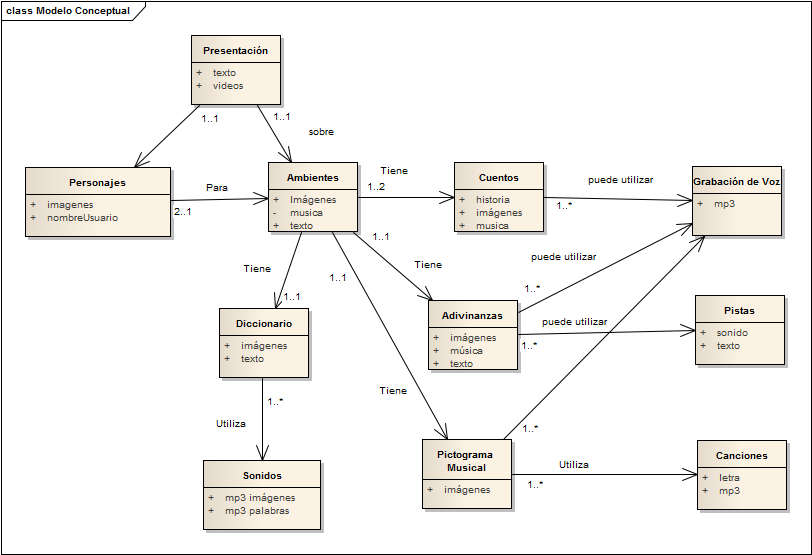
\includegraphics[width=14cm,height=10cm] {imagenes/ModeloConceptual.png}
	\end{center}
	\caption{Modelo Conceptual generado.}\label{concep}
\end{figure}



\vspace{1mm}
\subsection{Diagrama de Casos de Usos}

En el diagrama de caso de uso Figura \ref{diacaso}, veremos la funci�n de cada actor en el sistema, entendiendo el comportamiento que tendr� la aplicaci�n.

\begin{figure}[htf]
	\begin{center}
		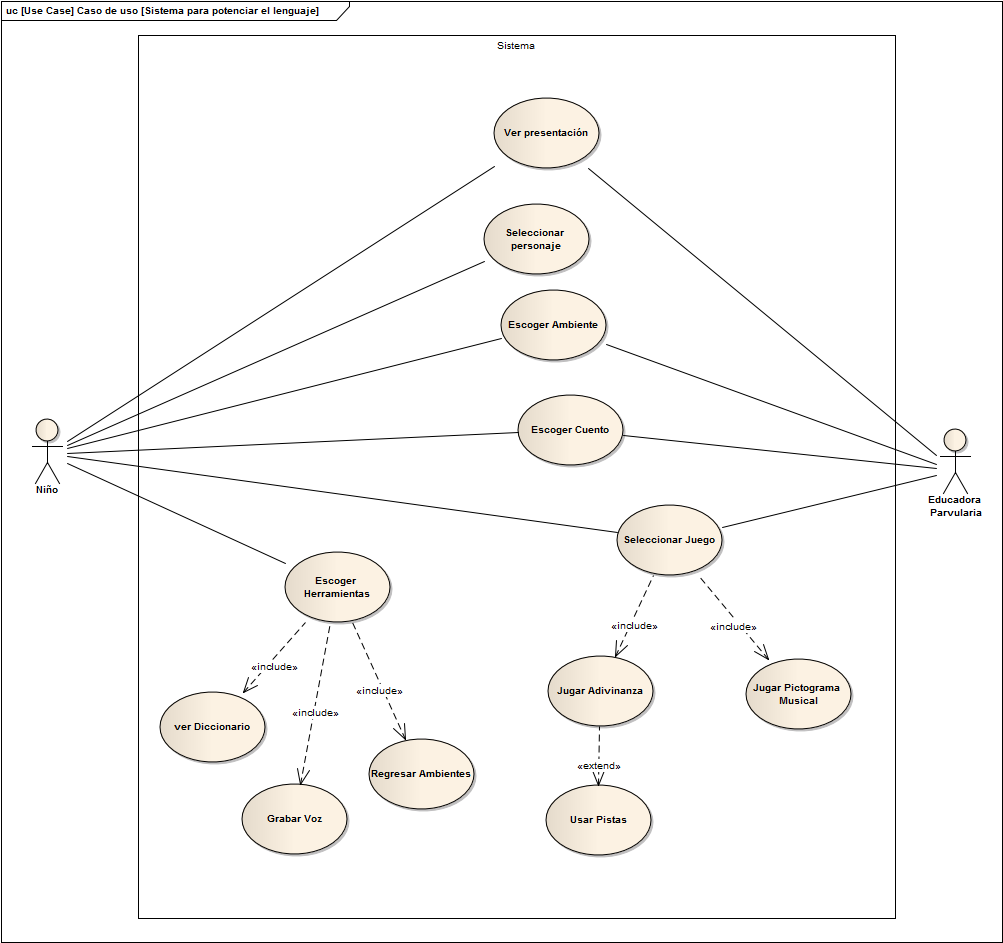
\includegraphics[width=16cm,height=12cm] {imagenes/CasosUsos.png}
	\end{center}
	\caption{Diagrama de Casos de Usos generado.}\label{diacaso}
\end{figure}


\clearpage
\newpage
\vspace{1mm}
\subsection{Casos de Usos Expandidos}

En esta secci�n se detallar� los casos de usos identificados en la Figura \ref{diacaso}, estableciendo la interacci�n entre los casos de usos y los requerimientos funcionales asociados a ellos.

\begin{table}[h]
	
	\begin{tabular}{rp{11cm}}
		
		{\bf Id} &      CU001 \\
		
		{\bf Nombre} &  Ver Presentaci�n  \\
		
		{\bf Actor} &   Ni�o, Educadora Parvularia. \\
		
		{\bf Prop�sito} & Ver la presentaci�n de la aplicaci�n y la introducci�n de las herramientas. \\
		
		{\bf Resumen} & El ni�o y la educadora podr�n ver la introducci�n de la aplicaci�n. \\
		
		{\bf Precondici�n} &     -       \\
		
		{\bf Ref. Cruzadas} &  REF008.      \\
		
		& \\
	\end{tabular}
	\begin{tabular}{|p{7cm}|p{7cm}|}
		\hline
		\multicolumn{2}{|c|}{{\bf Curso Normal}} \\
		\hline
		Actor &    Sistema \\
		\hline
		1. El ni�o / educadora presionar� empezar introducci�n. &            \\
		
		& 2. El sistema mostrar� un video explicativo sobre la introducci�n del juego y la explicaci�n de las herramientas. \\
		
		3. El ni�o / educadora finalizar� el video pulsando el bot�n siguiente.& \\
		
		& 4. Se procede al siguiente caso de uso.\\ \hline
		
		\multicolumn{2}{|c|}{{\bf Curso Alternativo }} \\
		\hline
		3 El ni�o / educadora volver� a ver nuevamente el video, seleccionando el bot�n volver a ver. & \\
		
		& 4 El sistema mostrar� nuevamente el video de presentaci�n. \\ \hline
		
	\end{tabular} 
	
	\caption{Caso de Uso Expandido: ver Presentaci�n.}\label{verpre}
\end{table}

Para obtener todas las espec�ficaciones de los casos de usos extendidos, visitar el \textbf{Ap�ndice A} adjuntado en este trabajo de t�tulo.

\vspace{1mm}


\clearpage
\newpage
\subsection{Diagramas de Secuencias}

\begin{figure}[htf]
	\begin{center}
		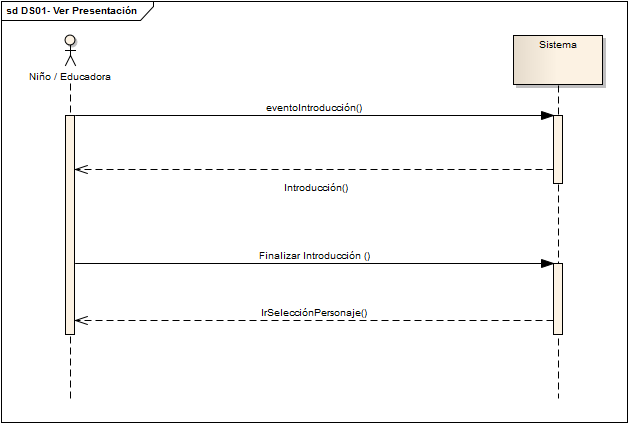
\includegraphics[width=10cm,height=8cm] {imagenes/DS01.png}
	\end{center}
	\caption{Caso de uso: Ver Presentaci�n}
\end{figure}

Para obtener todos los Diagramas de Secuencias, podr�n visitar el \textbf{Ap�ndice B} adjuntado en este trabajo de t�tulo.


\clearpage
\newpage
\vspace{1mm}
\subsection{Diagramas de Estados}


\begin{figure}[htf]
	\begin{center}
		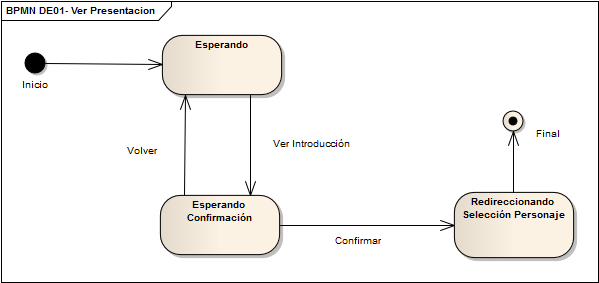
\includegraphics[width=13cm,height=6cm] {imagenes/DE01.png}
	\end{center}
	\caption{Caso de uso: Ver Presentaci�n}
\end{figure}

Para obtener todos los Diagramas de Estados, podr�n visitar el \textbf{Ap�ndice C} adjuntado en este trabajo de t�tulo.


\clearpage


\chapter{Dise�o}
\label{capdiseno}

\section{Dise�o del sistema a implementar}  \label{diseno}
En esta secci�n se presenta los distintos dise�os que representan el sistema a desarrollar, tanto en su arquitectura, su interfaz gr�fica, en el dise�o l�gico,  dise�o de datos y las pruebas de software a realizar.


\subsection{Dise�o arquitect�nico} \label{disenoarq}

Durante en la etapa de an�lisis se estableci� que la aplicaci�n ser� desarollada en dispositivos con sistema operativo Android, donde se implementa una arquitectura basada en android, la cual est� compuesta por 4 capas:

\begin{itemize}
	\item Aplicaciones
	\item Framework de Aplicaciones
	\item Biblioteca
	\item Kernel
\end{itemize}

\begin{figure}[htf]
	\begin{center}
		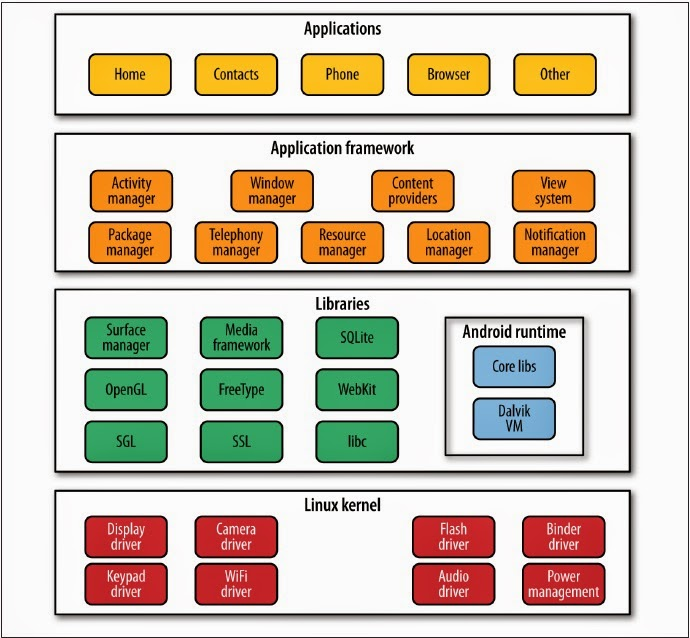
\includegraphics[width=9cm,height=9cm] {imagenes/arq.png}
	\end{center}
	\caption{Diagrama de arquitectura de Android.}
	\label{diarq1}
\end{figure}


\clearpage
\newpage
La Figura \ref{diarq1}  nos da a conocer que Android se encuentra construido a base del kernel de linux, pasando a la capa de librer�a qui�n se encarga de administrarlas en tiempo de ejecuci�n. Luego se encuentra la capa del framework que ayuda a construir la aplicaci�n que posteriormente es mostrada en la capa de aplicaciones \cite{arqui}.\\

Tomando en consideraci�n la arquitectura de android y los requerimientos analizados en la etapa de an�lisis, se establece la arquitectura del sistema a implementar.

\subsubsection{Diagrama de Arquitectura del Sistema}\label{arqsistema}

Para desarollar una aplicaci�n nativa en android, se ha establecido utilizar una arquitectura monol�tica, tambi�n conocido como arquitectura de una sola capa \cite{arqui2}.\\

La arquitectura de una sola capa (Figura \ref{diarq}), el sistema contiene las interfaces de usuario, la l�gica de negocio y los datos en el mismo equipo, administrado por el mismo sistema instalado en el equipo. Esto permite generar eficiencia en la comunicaci�n entre la interfaz, la l�gica y los datos en tiempo real, al momento de utilizar el sistema.

\begin{figure}[htf]
	\begin{center}
		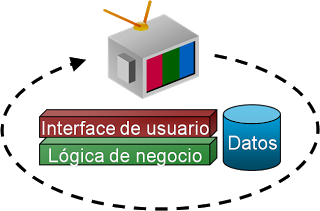
\includegraphics[width=8cm,height=6cm] {imagenes/arqsys.png}
	\end{center}
	\caption{Diagrama de arquitectura del sistema.}\label{diarq}
\end{figure}

\clearpage
\newpage
\subsection{Dise�o de interfaz} \label{disenointerfaz}

El dise�o de interfaz de usuario nos permite representar los requerimientos identificados en la etapa de an�lisis, utilizando prototipados en papel, para luego ser convertidos en prototipos digitales. A continuaci�n se presentar� el funcionamiento de la aplicaci�n a trav�s de la representaci�n ilustrativa de los prototipos obtenidos.

\subsubsection{Prototipo 1: Pantalla de Inicio }

En la primera pantalla de la aplicaci�n (Figura \ref{prot1}), deber� mostrar la introducci�n de la herramienta, explicando la finalidad y el enfoque de la aplicaci�n.\\

\begin{table}[h]
	
	\begin{tabular}{rp{11cm}}
		
		{\bf Id} &      CU001 \\
		
		{\bf Nombre} &  Ver Presentaci�n  \\
		
		{\bf Actor} &   Ni�o, Educadora Parvularia. \\
		
		{\bf Prop�sito} & Ver la presentaci�n de la aplicaci�n y la introducci�n de las herramientas. \\
		
		{\bf Resumen} & El ni�o y la educadora podr�n ver la introducci�n de la aplicaci�n. \\
		
		{\bf Precondici�n} &     -       \\
		
		{\bf Ref. Cruzadas} &  REF008.      \\
		
		& \\ 
	\end{tabular}
	\begin{tabular}{|p{7cm}|p{7cm}|}
		\hline
		\multicolumn{2}{|c|}{{\bf Curso Normal}} \\
		\hline
		Actor &    Sistema \\
		\hline
		1. El ni�o / educadora presionar� empezar introducci�n. &            \\
		
		& 2. El sistema mostrar� un video explicativo sobre la introducci�n del juego y la explicaci�n de las herramientas [\textbf{Punto A}, Figura \ref{prot1}].  \\
		
		3. El ni�o / educadora finalizar� el video pulsando el bot�n siguiente [\textbf{Punto B}, Figura \ref{prot1}].& \\ \hline
		
	\end{tabular} 
	\caption{Caso de Uso Expandido: ver Presentaci�n.}
\end{table}


\clearpage
\newpage 

\begin{figure}[htf]
	\begin{center}
		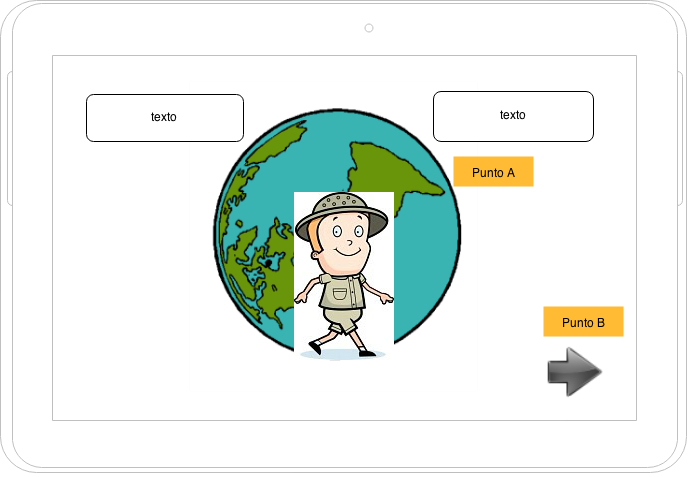
\includegraphics[width=9cm,height=5cm] {imagenes/pro1.png}
	\end{center}
	\caption{Prototipo 1, Pantalla de inicio} \label{prot1}
\end{figure}


Para un mayor detalles sobre los prototipos generados, podr�n acceder en el \textbf{Ap�ndice D}.



\clearpage
\newpage
\subsubsection{Diagrama de Navegaci�n}\label{dianave}

En el diagrama de navegaci�n (Figura \ref{fignave}), se presenta la secuencia de la utilizaci�n del sistema, accediendo a las funcionalidades espec�ficadas en la etapa de an�lisis del trabajo de t�tulo.


\begin{figure}[htf]
	\begin{center}
		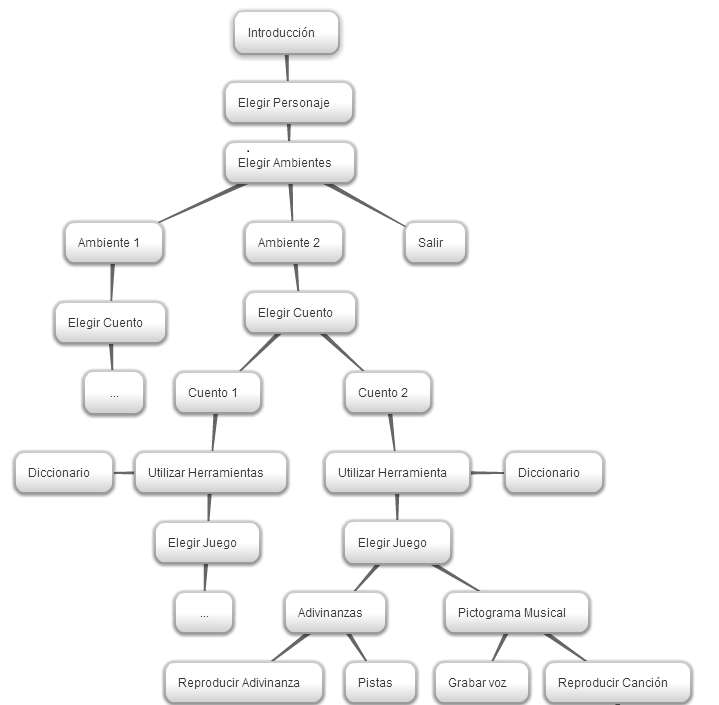
\includegraphics[width=12cm,height=13cm] {imagenes/diagramaNavegacion.png}
	\end{center}
	\caption{Diagrama de Navegaci�n}\label{fignave}
\end{figure}




\clearpage
\newpage
\subsection{Dise�o l�gico} \label{disenolog}

En el dise�o l�gico describiremos los requerimientos analizados, a trav�s de clases y objetos por utilizar en el desarrollo de la aplicaci�n.


\subsubsection{Diagrama de Clases}\label{diaclases}

Analizado el modelo conceptual de la etapa de an�lisis, se ha identificado las clases m�s importante del sistema, tal como se muestra en la figura \ref{diacla}.


\begin{figure}[htf]
	\begin{center}
		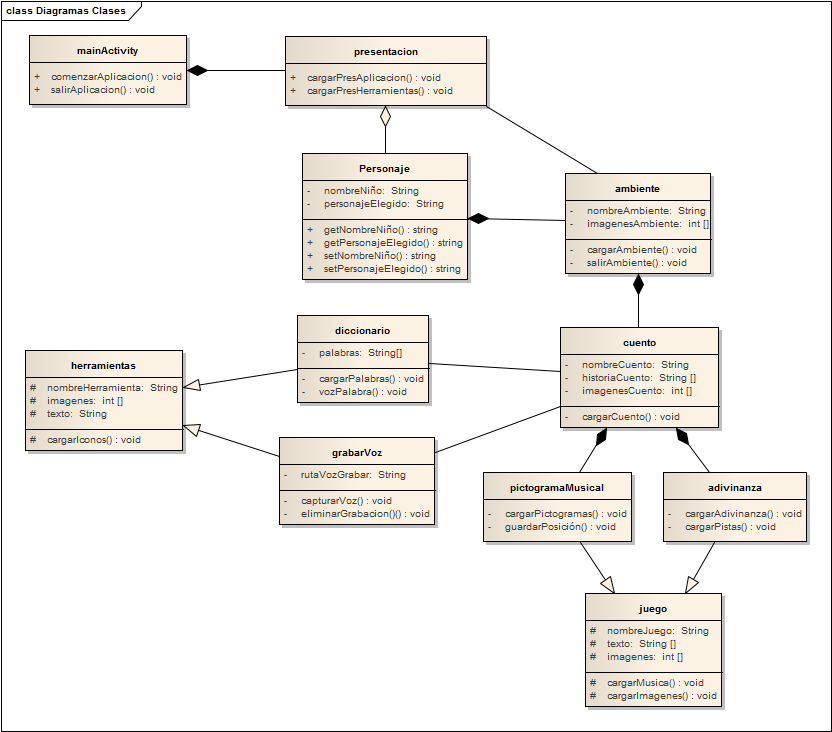
\includegraphics[width=16cm,height=14cm] {imagenes/clases.png}
	\end{center}
	\caption{Diagrama de clases del sistema} \label{diacla}
\end{figure}


\clearpage
\newpage
\subsubsection{Diagrama de Despliegue}\label{diadespliegue}

El sistema no cuenta con comunicaci�n de datos con otros nodos f�sicos (hardware).
La �nica interacci�n que existe, es el mismo nodo (dispositivo m�vil) que ejecuta la aplicaci�n a desarrollar.

\subsubsection{Diagrama de Componentes}\label{diaComponentes}

En el sistema a desarrollar, se ha logrado identificar 4 m�dulos compuestos por componentes en la figura \ref{figcom}, que los cuales son: 

\begin{itemize}
	
	\item \textbf{M�dulo Android:} Compuestos por componentes que contienen la l�gica del sistema, por ejemplo, la creaci�n de ambientes, cuentos y juegos. 
	
	\item \textbf{M�dulo Libraries Android:} Biblioteca de Android que facilitan los recursos de interfaz y funcionalidades  de Android, por ejemplo, librer�a de utilizaci�n del micr�fono, creaci�n de botones, reproducci�n de m�sica y sonido, entre otras \cite{libreria}.
	
	\item \textbf{M�dulo Config:} M�dulo que establece los archivos de configuraci�n del sistema, por ejemplo, los dispositivos compatibles, los permisos de utilizaci�n de funcionalidades de android.
	
	\item \textbf{M�dulo Execute:} M�dulo que contiene el archivo ejecutable de la instalaci�n de la aplicaci�n.
	
\end{itemize}

\begin{figure}[htf]
	\begin{center}
		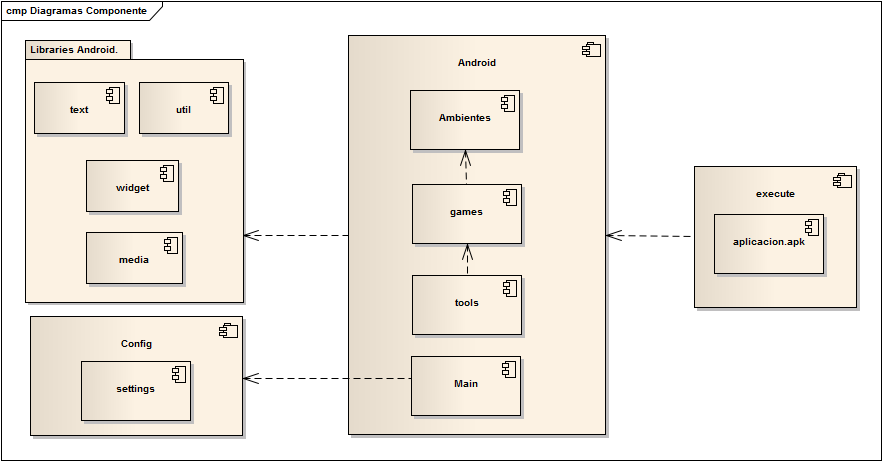
\includegraphics[width=14cm,height=12cm] {imagenes/comp.png}
	\end{center}
	\caption{Diagrama de componentes del sistema.} \label{figcom}
\end{figure}

\clearpage
\newpage


\subsection{Dise�o de datos}  \label{disenodatos}

Dentro de la aplicaci�n a desarrollar, no se ocupar� una base de datos que almacene informaci�n del usuario o del sistema, ya que solamente se rescatar� los pocos recursos integrados en la aplicaci�n, tales como: 

\begin{itemize}
	
	\item \textbf{Im�genes:} Fondos, pictogramas, botones y dibujos.
	\item \textbf{Archivos de texto:} Nombre del ni�o, letras y textos.
	\item \textbf{M�sica:} M�sica de fondo, sonidos de botones y canciones.
	
\end{itemize}


\subsection{Dise�o de pruebas}\label{disenopruebas}

En el dise�o de pruebas se especifican todas las pruebas que se realizar�n al sistema una vez implementado, con el objetivo de corregir los problemas que pueden presentar desde el momento de la instalaci�n de la aplicaci�n, hasta y durante la ejecuci�n del sistema.\\

El dise�o de pruebas ser� aplicado en el siguiente orden:

\begin{itemize}
	\item Pruebas Unitarias
	\item Pruebas de Integraci�n
	\item Pruebas de Usabilidad
	\item Pruebas de Aceptaci�n y Rechazo.
\end{itemize}

\clearpage
\newpage
\subsubsection{Pruebas Unitarias}\label{puebasunitarias}

Las pruebas unitarias consisten en realizar revisiones en peque�os fragmentos de c�digo del sistema \cite{pruebau}. Estos fragmentos representan a tareas at�micas de caracter espec�ficos e independientes, en el sistema por desarrollar.\\

Las pruebas unitarias permiten simplificar las pruebas de integraci�n, fomentar a la refactorizaci�n y documentaci�n del c�digo.\\
El tipo de prueba utilizar, ser� el m�todo de "caja negra".\\

El m�todo de caja negra son pruebas funcionales donde se define un conjunto de condiciones de entradas que abarcan los requisitos funcionales del sistema.\\
Las pruebas de caja negra establecen un conjunto de entradas y las salidas esperadas, no importando el interior del sistema.\\


La plantilla utilizada para realizar las pruebas unitarias es la Tabla \ref{tablapuplantilla}

\begin{table}[htf]
	
	\centering
	\begin{tabular}{|p{4cm}|p{7cm}|}
		\hline
		\multicolumn{ 2}{|c|}{{\bf PU001: XXXX}} \\\hline
		\textbf{Prop�sito:} &  \\ \hline 
		\textbf{Caso de Uso:} &  \\ \hline
		
		\multicolumn{2}{|c|}{{\textbf{Caso prueba}}} \\ 	\hline
		\textbf{Entradas:} &  \\ \hline
		
		\textbf{Salida Esperada:} &  \\ \hline
		
		\multicolumn{2}{|c|}{{\textbf{Valores de caso prueba}}} \\ 	\hline
		\textbf{Entrada }& \textbf{Salida} \\ \hline
		
		& \\ \hline
		&  \\ \hline
		
	\end{tabular} 
	\caption{Tabla de plantilla de las pruebas unitarias}\label{tablapuplantilla}	
\end{table}

A partir de la Tabla \ref{tablapuplantilla}, se obtienen las pruebas unitarias que son las siguientes: 

\clearpage
\newpage
\begin{table}[htf]
	
	\centering
	\begin{tabular}{|p{4cm}|p{7cm}|}
		\hline
		\multicolumn{ 2}{|c|}{{\bf PU001: Drag and drop}} \\\hline
		\textbf{Prop�sito:} & Generar el movimiento de drag and drop en el sistema \\ \hline 
		\textbf{Caso de Uso:} & CU008\\ \hline
		
		\multicolumn{2}{|c|}{{\textbf{Caso prueba}}} \\ 	\hline
		\textbf{Entradas:} & x,y Valores enteros de imagen \\ \hline
		
		\textbf{Salida Esperada:} & Posici�n x,y de la imagen \\ \hline
		
		\multicolumn{2}{|c|}{{\textbf{Valores de caso prueba}}} \\ 	\hline
		\textbf{Entrada }& \textbf{Salida} \\ \hline
		
		x=400; y=500 & Imagen en x=400; y=500 (Correcto)\\ \hline
		x=600; y=700 & Imagen en x=600; y=700 (Correcto) \\ \hline
		
	\end{tabular} 
	\caption{Tabla de Pruebas Unitarias PU001}\label{tablapu001}	
\end{table}


En el \textbf{Ap�ndice E} se encuentran el dise�o de pruebas unitarias restantes.



\clearpage
\newpage
\subsubsection{Pruebas de Integraci�n}\label{prueintegrar}  

Las pruebas de integraci�n corresponde al conjunto de tareas espec�ficas que han sido ejecutadas en las pruebas de unitarias, donde establecen dos o m�s interacciones entre ellas. Estas pruebas pueden ser clases, m�dulos, paquetes, subsistemas, entre otras.\\
Las pruebas de integraci�n tienen como objetivo verificar las funciones y rendimiento de ellas \cite{pruebai}.\\

Los tipos de pruebas de integraci�n son las siguientes:


\begin{itemize}
	
	\item \textbf{Top-Down}: Consiste en empezar a integrar los m�dulos o subsistemas m�s importantes del sistema, realizando las pruebas hacia los niveles inferiores.
	
	\item \textbf{Bottom-Up}: Consiste en realizar las pruebas en los m�dulos de niveles inferiores de abstracci�n, apuntando a los niveles con m�s abstracci�n del sistema.
	
	\item \textbf{Big - Bang}: Consiste en probar todos los m�dulos desarrollados en conjunto, recreando la mayor parte del sistema. Tiene como finalidad ahorrar el tiempo dedicado en realizar las pruebas de Top-Down y Bottom-up, pero el proceso de integraci�n es m�s complicado por su acoplamiento existente entre los modulos testeados.
	
\end{itemize}

Las pruebas de integraci�n a utilizar es \textbf{Bottom-up} (Figura \ref{buttonup} ), porque permite detectar eficazmente las funcionalidades que no se encuentran ejecut�ndose correctamente, escalando hasta los niveles m�s abstractos del sistema.


\begin{figure}[h]
	\begin{center}
		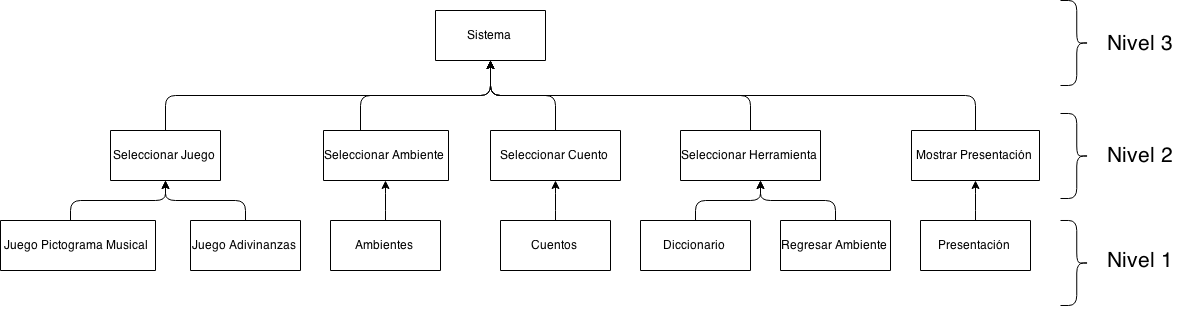
\includegraphics[width=16cm,height=7cm] {imagenes/bottonup.png}
	\end{center}
	\caption{Diagrama de la prueba integraci�n Bottom-UP} \label{buttonup}
\end{figure}

\clearpage
\newpage

La plantilla utilizada para las pruebas de integraci�n corresponde a la Figura \ref{tablapiplantilla}:\\

\begin{table}[htf]
	
	\centering
	\begin{tabular}{|p{3.5cm}|p{7cm}|}
		
		\hline
		\multicolumn{ 2}{|c|}{{\bf PI001: XXXX }} \\\hline
		Nivel: &   \\ \hline 
		Objetivo:&	\\ \hline
		Estado Inicial: &  \\ \hline
		Estado Final: &  \\ \hline
		Resultado Esperado: &   \\ \hline
		Resultado   Obtenido:&  \\ \hline
		
	\end{tabular} 
	\caption{Tabla de Plantilla para lasPruebas de Integraci�n}\label{tablapiplantilla}
	
\end{table}

A partir de la Figura \ref{tablapiplantilla}, se realizar�n las siguientes pruebas de integraci�n:\\

\begin{table}[htf]
	
	\centering
	\begin{tabular}{|p{3.5cm}|p{7cm}|}
		
		\hline
		\multicolumn{ 2}{|c|}{{\bf PI001: Juego Pictograma Musical }} \\\hline
		Nivel: &  1\\ \hline 
		Objetivo:& Arrastrar Im�genes en la letra de la canci�n, reproducir la canci�n y grabaci�n de la voz.  \\ \hline
		Estado Inicial: & Inicializar interfaz del juego y en espera de usar las funcionalidades  \\ \hline
		Estado Final: & Usar todas las im�genes y la grabaci�n de voz  \\ \hline
		Resultado Esperado: &  Im�genes en la posici�n correcta, completando el juego. Pasar al otro juego  \\ \hline
		Resultado   Obtenido:& -\\ \hline
		
	\end{tabular} 
	\caption{Tabla de Pruebas de Integraci�n - PI001}\label{tablapi001}
	
\end{table}

Para un mayor detalle de las Pruebas de Integraci�n, podr�n acceder al \textbf{Ap�ndice F} adjuntado en este trabajo de t�tulo.


\clearpage
\newpage
\subsubsection{Pruebas de Usabilidad}\label{prueusable}

Las pruebas de usabilidad son centradas en el usuario que permiten evaluar si el sistema puede realmente cumplir con las tareas del sistema, en t�rminos de efectividad, eficiencia y satisfacci�n \cite{pruebausa}.\\

Una de las t�cnicas de usabilidad m�s utilizadas, corresponde a la evaluaci�n heur�stica establecidas por Jacob Nielsen.\\

La evaluaci�n heur�stica tiene como objetivo de inspeccionar la interfaz de la aplicaci�n para descubrir los problemas potenciales de usabilidad \cite{heu1}.\\
La evaluaci�n heur�stica es una t�cnica cualitativa que consiste en evaluar la conformidad de la interfaz del sistema .\\

Los puntos m�s importantes utilizados en la evaluaci�n heur�stica (Figura \ref{tablahe3} y \ref{tablahe4}) son los siguientes \cite{heu2}:


\begin{table}[htf]
	\centering
	\begin{tabular}{|p{5cm}|p{7cm}|}
		
		\hline
		\textbf{Nombre} & \textbf{Descripci�n} \\ \hline 
		1- Visibilidad del estado del sistema & El sistema debe mantener informado al usuario sobre las acciones que estan ocurriendo en el sistema.  \\ \hline
		2- Similitud entre el sistema y el mundo real & El sistema debe hablar en le lenguaje del usuario.  \\ \hline
		3- Control y libertad del usuario & El sistema debe presentar una opci�n para volver a la acci�n anterior, en caso que el usuario se equivoque en su elecci�n.  \\ \hline
		4- Consistencia y est�ndares & Los usuarios no deben cuestionar acciones o situaciones, siguiendo conveciones y normas del sistema. \\ \hline
		5- Prevenci�n de errores  & Eliminar y corregir los posibles problemas que con llevan errores.\\ \hline
		6- Reconocimiento en vez de recordar & Dejar visible los objetos, acciones y opciones. El usuario no debe preguntarse al recordar informaci�n espec�fica.\\ \hline
		7- Flexibilidad y Eficiencia de uso & Entregar aceleradores que permitan aumentar la velocidad de interacci�n para usuarios expertos y novatos. \\ \hline
	\end{tabular} 
	\caption{Tabla de heur�sticas}\label{tablahe3}
	
\end{table}



\clearpage
\newpage

\begin{table}
	\centering
	\begin{tabular}{|p{5cm}|p{7cm}|}
		
		\hline
		\textbf{Nombre} & \textbf{Descripci�n} \\ \hline 
		8- Est�tica y dise�o minimalista & La interfaz no debe contener informaci�n irrelevante, disminuyendo la visibilidad de la interfaz. \\ \hline
		9- Ayuda ante errores & El mensaje de error debe ser claro, indicando el problema. \\ \hline
		10- Ayuda y documentaci�n & En el caso de utilizar, �sta debe ser f�cil de encontrar y centrada a las tareas del usuario. \\ \hline
		
	\end{tabular} 
	\caption{Tabla de heur�sticas}\label{tablahe4}
	
\end{table}


A partir de las heur�sticas establecidas en la figura \ref{tablahe3}, se aplicar�n las plantillas de la tabla de escala de severidad (Figura \ref{tablahe}) y de la tabla de frecuencia de severidad (Figura), entregando datos cuantitativos de la evaluaci�n.\\


\begin{table}[htf]
	
	\centering
	\begin{tabular}{|p{4cm}|p{4cm}|p{4cm}|}
		
		\hline
		\textbf{Clasificaci�n} & \textbf{Severidad} & \textbf{Correcci�n}\\ \hline 
		
		\centering 4 & Problema Catastr�fico & Vital \\ \hline
		\centering 3 & Problema Alto& Alto \\ \hline
		\centering 2 & Problema Menor& Bajo \\ \hline
		\centering 1 & Problema c�smetico& Muy bajo\\ \hline
		\centering 0 & No es un problema& - \\ \hline
		
	\end{tabular} 
	\caption{Tabla de escala de severidad}\label{tablahe}
	
\end{table}


\begin{table}[htf]
	\centering
	\begin{tabular}{|p{4cm}|p{4cm}|}
		
		\hline
		\textbf{Clasificaci�n} & \textbf{Frecuencia} \\ \hline 
		\centering 4 &  90\% - 100\% \\ \hline
		\centering 3 &  51\% - 89\% \\ \hline
		\centering 2 &  11\% - 50\% \\ \hline
		\centering 1 &  2\% - 10\% \\ \hline
		\centering 0 & 1\%	\\ \hline
		
	\end{tabular} 
	\caption{Tabla de frecuencia de severidad}\label{tablahe2}
	
\end{table}


\clearpage
\newpage
\subsubsection{Pruebas de Aceptaci�n y de Rechazo de los Usuarios}\label{prueacepta}

Las pruebas de aceptaci�n de usuarios tienen como finalidad de corroborar los requerimientos obtenidos del usuario.\\
El usuario nos entrega la informaci�n sobre el sistema, si cumple las tareas y objetivos establecidos a comienzo del desarrollo de la aplicaci�n.\\
La educadoras parvularias realizar�n estas pruebas de aceptaci�n y rechazo.\\

En la tabla \ref{encuestaEducadora} y \ref{encuestaEducadora2} se espec�fica los t�picos que integrar� esta prueba.\\


\begin{table}[htf]
	\begin{tabular}{|p{10.5cm}|lllll|}
		\hline
		\textbf{Item} & 1 & 2 & 3 & 4 & 5 \\
		\hline
		\multicolumn{6}{|l|}{\textbf{Actividades}}\\
		\hline
		1.La elecci�n de ambientes, permite diversificar el contenido de aplicaci�n.  &  $\bigcirc $ &  $\bigcirc $ &  $\bigcirc $ &  $\bigcirc $ &  $\bigcirc $ \\
		2. Los cuentos son atractivos, cortos y f�ciles de entender. &  $\bigcirc $ &  $\bigcirc $ &  $\bigcirc $ &  $\bigcirc $ &  $\bigcirc $\\
		3. Las adivinanzas es f�cil e intuitivo. &  $\bigcirc $ &  $\bigcirc $ &  $\bigcirc $ &  $\bigcirc $ &  $\bigcirc $\\
		4. Las adivinanzas entrega pistas que ayudan a resolver la adivinanza. &  $\bigcirc $ &  $\bigcirc $ &  $\bigcirc $ &  $\bigcirc $ &  $\bigcirc $\\
		5. El pictograma musical es f�cil e intuitivo. &  $\bigcirc $ &  $\bigcirc $ &  $\bigcirc $ &  $\bigcirc $ &  $\bigcirc $\\
		6. El pictograma musical permite grabar la voz en conjunto a la pista de la canci�n. &  $\bigcirc $ &  $\bigcirc $ &  $\bigcirc $ &  $\bigcirc $ &  $\bigcirc $\\  
		\hline
		\multicolumn{6}{|l|}{\textbf{Funcionalidades}}\\
		\hline
		7. La funci�n de arrastrar y soltar en pictograma musical, funciona correctamente. &  $\bigcirc $ &  $\bigcirc $ &  $\bigcirc $ &  $\bigcirc $ &  $\bigcirc $\\
		8. Los botones presenten en la aplicaci�n, todos tienen una funcionalidad asociada correctamente. &  $\bigcirc $ &  $\bigcirc $ &  $\bigcirc $ &  $\bigcirc $ &  $\bigcirc $\\
		8. Se muestra las presentaciones que introducen el juego y las herramientas. &  $\bigcirc $ &  $\bigcirc $ &  $\bigcirc $ &  $\bigcirc $ &  $\bigcirc $\\
		\hline
		
	\end{tabular}
	\caption{Encuesta Educadora Parvularia} \label{encuestaEducadora}
\end{table}

\clearpage
\newpage 

\begin{table}[H]
	\begin{tabular}{|p{10.5cm}|lllll|}
		\hline
		\textbf{Item} & 1 & 2 & 3 & 4 & 5 \\
		
		\hline
		\multicolumn{6}{|l|}{\textbf{Herramientas}} \\
		\hline
		9. Todos los �conos que pertenece a la barra de herramientas acceden a su funci�n. &  $\bigcirc $ &  $\bigcirc $ &  $\bigcirc $ &  $\bigcirc $ &  $\bigcirc $\\
		10. El �cono de lupa, entrega la pantalla de palabras con sus significados e im�genes. &  $\bigcirc $ &  $\bigcirc $ &  $\bigcirc $ &  $\bigcirc $ &  $\bigcirc $\\
		11. El �cono del planeta tierra regresa a la pantalla principal de la aplicaci�n. &  $\bigcirc $ &  $\bigcirc $ &  $\bigcirc $ &  $\bigcirc $ &  $\bigcirc $\\
		12. El �cono de la grabaci�n de voz, permite ejecutar su funcionalidad. &  $\bigcirc $ &  $\bigcirc $ &  $\bigcirc $ &  $\bigcirc $ &  $\bigcirc $\\
		13. El �cono de la doble corchea, permite silenciar y activar la m�sica de la aplicaci�n. &  $\bigcirc $ &  $\bigcirc $ &  $\bigcirc $ &  $\bigcirc $ &  $\bigcirc $\\
		\hline
		
		
		\multicolumn{6}{|l|}{\textbf{Multimedia}}\\
		\hline
		14. Los sonidos, canciones y grabaciones estan asociados correctamente en la aplicaci�n. &  $\bigcirc $ &  $\bigcirc $ &  $\bigcirc $ &  $\bigcirc $ &  $\bigcirc $\\
		15. En la cantidad de im�genes y sonidos son variados. &  $\bigcirc $ &  $\bigcirc $ &  $\bigcirc $ &  $\bigcirc $ &  $\bigcirc $\\
		16. Las im�genes son utilizadas correctamente en el contexto de la pantalla donde se encuentra. &  $\bigcirc $ &  $\bigcirc $ &  $\bigcirc $ &  $\bigcirc $ &  $\bigcirc $\\
		17. El movimiento del planeta tierra se ve correctamente en la presentaci�n y en la pantalla principal. &  $\bigcirc $ &  $\bigcirc $ &  $\bigcirc $ &  $\bigcirc $ &  $\bigcirc $\\
		18. La calidad de la im�genes y sonidos son acordes a la aplicaci�n. &  $\bigcirc $ &  $\bigcirc $ &  $\bigcirc $ &  $\bigcirc $ &  $\bigcirc $\\
		\hline
		
		\multicolumn{6}{|l|}{\textbf{Importancia}}\\
		\hline
		19. El ni�o/a realiza las actividades f�cilmente. &  $\bigcirc $ &  $\bigcirc $ &  $\bigcirc $ &  $\bigcirc $ &  $\bigcirc $\\
		20. La aplicaci�n funciona correctamente. &  $\bigcirc $ &  $\bigcirc $ &  $\bigcirc $ &  $\bigcirc $ &  $\bigcirc $\\
		21. La aplicaci�n es una herramienta alternativa importante en el desarrollo del lenguaje . &  $\bigcirc $ &  $\bigcirc $ &  $\bigcirc $ &  $\bigcirc $ &  $\bigcirc $\\
		22. La aplicaci�n deber� incluir m�s actividades, m�s ambientes, para diversificar a�n m�s su contenido. &  $\bigcirc $ &  $\bigcirc $ &  $\bigcirc $ &  $\bigcirc $ &  $\bigcirc $\\
		\hline
	\end{tabular}
	\caption{Encuesta Educadora Parvularia} \label{encuestaEducadora2}
\end{table}
\chapter{Implementaci�n}
\label{capimplementacion}
En esta secci�n se abordar�n  las herramientas utilizadas durante el desarrollo de la aplicaci�n, entregando  las especificaciones t�cnicas  y la descripci�n de cada una de ellas. 


\section{Herramientas de Software}\label{herraSoftware}

Para el desarrollo de la aplicaci�n, se ocup� un entorno de desarrollo ligero formado por el editor de texto \textbf{Sublime Text}\cite{sublime} y el plugin \textbf{Corona editor}\cite{fuse}.

\begin{itemize}
	
\item \textbf{Sublime Text 3.0} : Editor de texto gratuito sofisticado que permite escribir el c�digo del programa. Adem�s es extensible, permitiendo la integraci�n de plugins que ayuden a configurar nuestro IDE.

\item \textbf{Corona Editor} : Plugin gratuito para Sublime Text instalable desde el package control plugin de Sublime Text.\\
Corona Editor entrega herramientas de depuraci�n, debugueo, completaci�n de c�digo, documentaci�n, consola y compilaci�n de c�digo. 
	
\end{itemize}


\section{Hardware de Desarrollo}\label{hardDesarrollo}

Para desarrollar el programa se utiliz� el siguiente equipo con las siguientes especificaciones t�cnicas:

\begin{itemize}

\item \textbf{Modelo}: Samsung GALAXY Tab 2 (7.0)
\item \textbf{Tama�o}: 600 x 1024 pixels, 7.0 pulgadas
\item \textbf{Memoria}: 1GB RAM
\item \textbf{Procesador}: Procesador dual core 1GHz
\item \textbf{Almacenamiento}: 8GB
\item \textbf{Sistema Operativo}: Android OS, v4.0 Ice Cream Sandwich

\end{itemize}




\section{Lenguajes de Programaci�n}\label{lengProgra}

El lenguaje de programaci�n utilizado para desarrollar el trabajo de t�tulo est� determinado por el framework seleccionado, que corresponde al lenguaje \textbf{Lua} \cite{lua}.\\


Lua, es un lenguaje de programaci�n extensible dise�ado para una programaci�n procedimental con utilidades para la descripci�n de datos.
Ofrece soporte para la programaci�n orientada a objeto, programaci�n funcional y programaci�n orientada a datos.\\

Lua es usado como un lenguaje de script potente y ligero para cualquier programa que lo necesite, implementado con las librer�as escritas en el lenguaje C.\\

Adem�s, Lua es un lenguaje robusto probado y utilizado en muchas aplicaciones, como por ejemplo, MySQL Worbench y  VLC media player. \\
Tambi�n es utilizado principalmente en la construcci�n y desarrollo de juegos, por ejemplo:


\begin{itemize}
	
	\item Angry Birds
	\item Crysis
	\item Farcry
	\item L.A Noire
	\item The Witcher
	\item World of Warcraft
	
\end{itemize}


\clearpage
\newpage
\section{Framework}\label{frameLib}

El framework elegido corresponde a \textbf{Corona SDK} \cite{corona}.\\

\textbf{Corona SDK} es un framework ocupado esencialmente para la creaci�n de juegos para dispositivos m�viles. Se basa en el lenguaje de programaci�n Lua de f�cil aprendizaje, que en conjunto de APIs, permiten a�adir caracter�sticas con pocas l�neas de c�digo.\\

\textbf{Corona SDK} permite publicar para iOS, Android, Kindle Fire, Nook y Windows 8 Phone, a partir de una sola base de c�digo.\\

Se ha escogido el framework \textbf{Corona SDK}, por las siguientes razones:

\begin{itemize}
	
	\item \textbf{Integraci�n de OpenGL-ES}: Permite utilizar funcionalidades que manipulen la pantalla del programa, permitiendo crear la funcionalidad drag and drop, detectar choques de objetos en tiempo de ejecuci�n y la creaci�n de animaciones a trav�s de pocas l�neas de c�digo.
	
	\item \textbf{Desarrollo de multiplataforma}: Corona nos permite crear aplicaciones tanto para iOS (iPhone y iPad) como tambi�n en m�viles Android.
	
	\item \textbf{Rendimiento}: Corona est� optimizado para hacer uso de las caracter�sticas de hardware aceleraci�n, dando como resultado un alto rendimiento en juegos y aplicaciones.
	
	\item \textbf{Caraster�sticas del dispositivo}: Posee acceso y control del dispositivo y del hardware, como por ejemplo, c�mara, aceler�metro, GPS y especialmente el acceso al micr�fono, utilizado en el desarrollo de la aplicaci�n del trabajo de t�tulo.
	
	
	\item \textbf{Nivel de aprendizaje}: Corona utiliza el lenguaje Lua que es potente y  f�cil de aprender.
	
	\item \textbf{Documentaci�n}: Corona tiene una comunidad donde ayuda a los desarrolladores a resolver problemas, aportar funcionalidades desarrolladas en sus aplicaciones. Adem�s cuenta con la espec�ficaci�nd de cada una de sus librer�as, con ejemplos que ayudan a construir la aplicaci�n r�pidamente. 
	
	
	\item \textbf{Licencia}: Corona SDK tiene una licencia gratuita, que nos permite publicar sin ning�n problema en tiendas de car�cter comerciales, como por ejemplo Google Play.
	
	
\end{itemize}



\clearpage
\newpage
\section{Interfaces del Sistema}\label{interSis}

Durante la etapa de implementaci�n se obtuvieron las siguientes interfaces:


\subsubsection{Introducci�n de la aplicaci�n}

En esta pantalla se da comienzo a la aplicaci�n, entregando la tem�tica que se desarrollar� durante la historia (Figura\ref{intApli}) .

\begin{figure}[htf]
	\begin{center}
		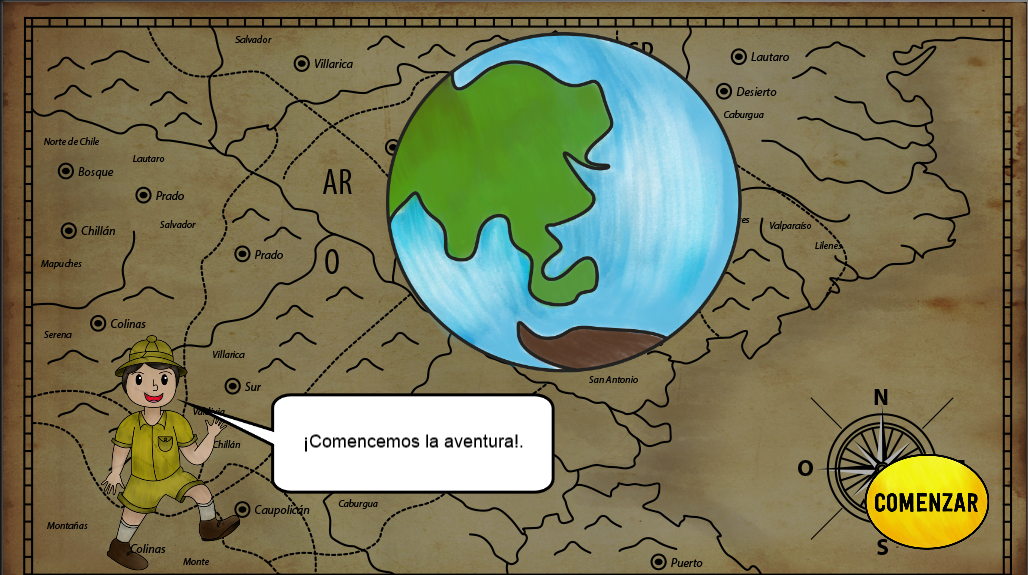
\includegraphics[width=12cm,height=6cm] {imagenes/introduccion.PNG}
	\end{center}
	\caption{Introducci�n a la aplicaci�n.}\label{intApli}
\end{figure}

\clearpage
\newpage
\subsubsection{Selecci�n de Personaje}

El usuario podr� elegir su personaje, teniendo la posibilidad de elegir entre ni�o o ni�a (Figura\ref{selPer}) .

\begin{figure}[htf]
	\begin{center}
		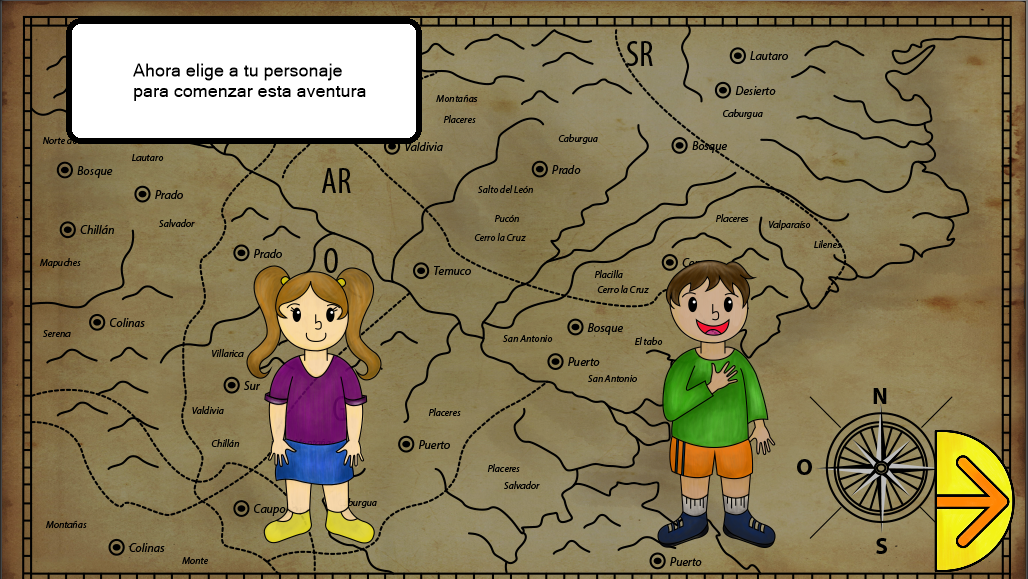
\includegraphics[width=12cm,height=6cm] {imagenes/seleccionPersonaje.PNG}
	\end{center}
	\caption{Selecci�n de Personaje.}\label{selPer}
\end{figure}


\subsubsection{Selecci�n de Ambiente}

En esta pantalla se explicar� el ambiente Sabana, indicando sus caracter�sticas generales de ella (Figura\ref{selAmb}) .

\begin{figure}[htf]
	\begin{center}
		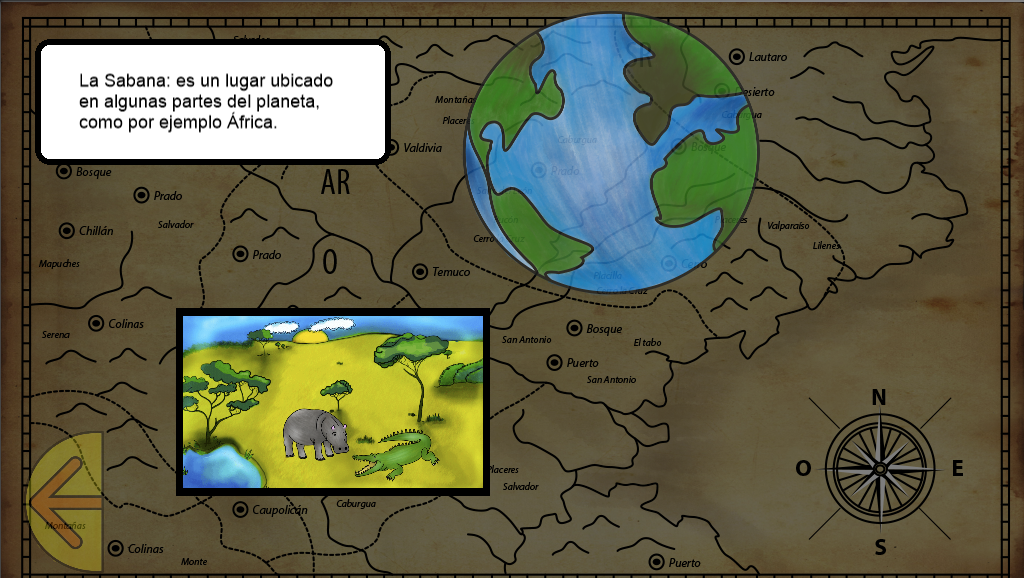
\includegraphics[width=12cm,height=6cm] {imagenes/seleccionAmbiente.PNG}
	\end{center}
	\caption{Selecci�n de Ambiente.}\label{selAmb}
\end{figure}
  
\clearpage
\newpage
\subsubsection{Introducci�n de herramientas}

En esta pantalla se explicar� la funcionalidad de las herramientas de la aplicaci�n, encontrando el diccionario, la m�sica y el planeta (Figura\ref{intHer}).

\begin{figure}[htf]
	\begin{center}
		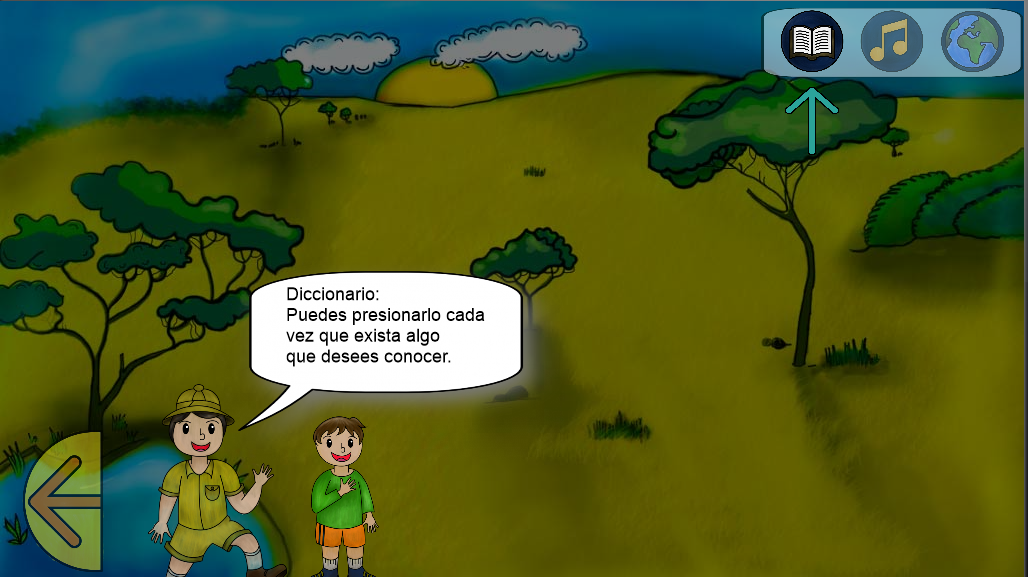
\includegraphics[width=12cm,height=6cm] {imagenes/herramientas.PNG}
	\end{center}
	\caption{Introducci�n de herramientas.}\label{intHer}
\end{figure}

\subsubsection{Selecci�n de cuentos}

El usuario podr� elegir dos cuentos disponible en el ambiente, en donde podr� obtener dos historias diferentes basadas en la Sabana (Figura\ref{selCue}).

\begin{figure}[htf]
	\begin{center}
		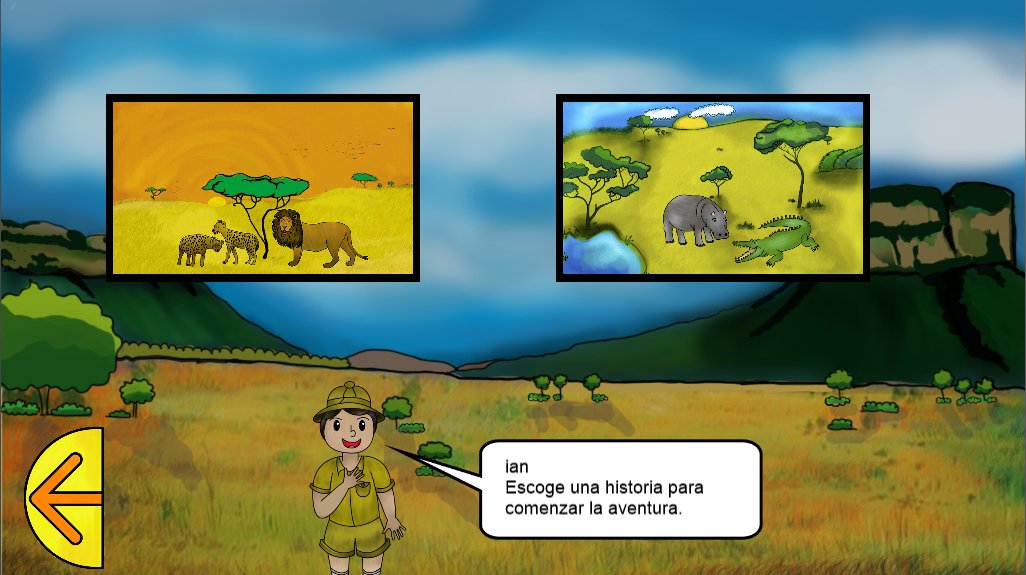
\includegraphics[width=12cm,height=6cm] {imagenes/seleccionCuentos.PNG}
	\end{center}
	\caption{Selecci�n de Cuentos.}\label{selCue}
\end{figure}

\clearpage
\newpage
\subsubsection{Cuentos}

En estas pantallas se contar� dos historias diferentes ambientado en la Sabana, que a partir de ellas, se realizar�n los juegos de la aplicaci�n. (Figura\ref{Cue1} y Figura\ref{Cue2}).

\begin{figure}[htf]
	\begin{center}
		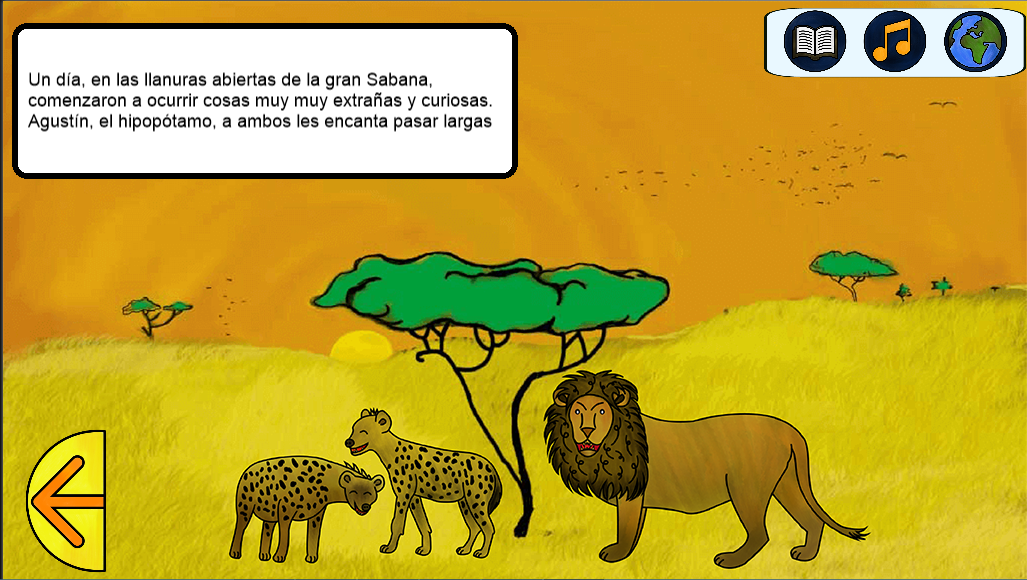
\includegraphics[width=12cm,height=6cm] {imagenes/cuento1.PNG}
	\end{center}
	\caption{Cuento1: Algo extra�o sucede en la sabana.}\label{Cue1}
\end{figure}

\begin{figure}[htf]
	\begin{center}
		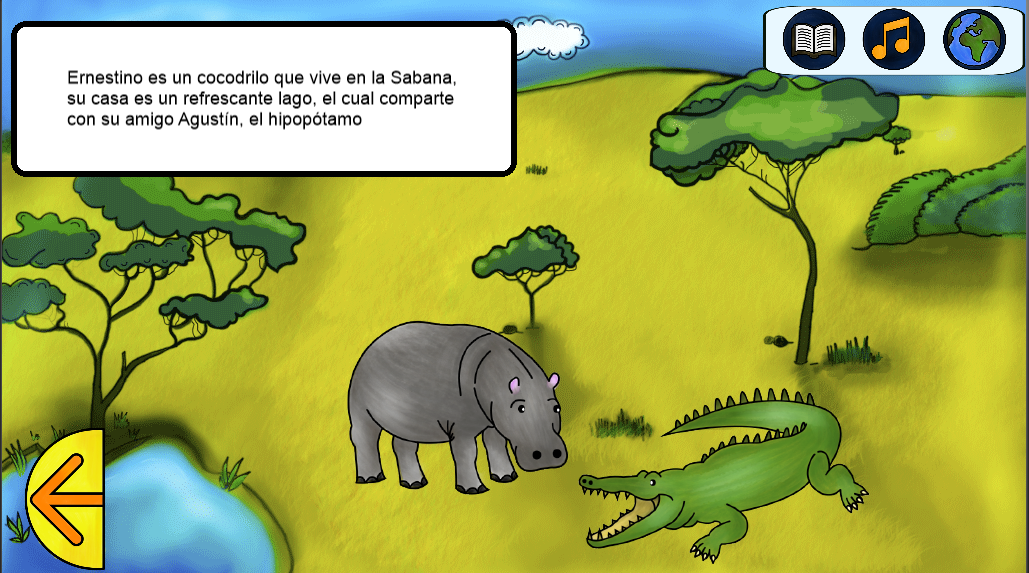
\includegraphics[width=12cm,height=6cm] {imagenes/cuento2.PNG}
	\end{center}
	\caption{Cuento2: Un paseo por la sabana.}\label{Cue2}
\end{figure}

\clearpage
\newpage
\subsubsection{Selecci�n de Juegos}

En la selecci�n de juegos podremos elegir entre los juegos de adivinanzas y pictograma musical. (Figura\ref{selJue}).

\begin{figure}[htf]
	\begin{center}
		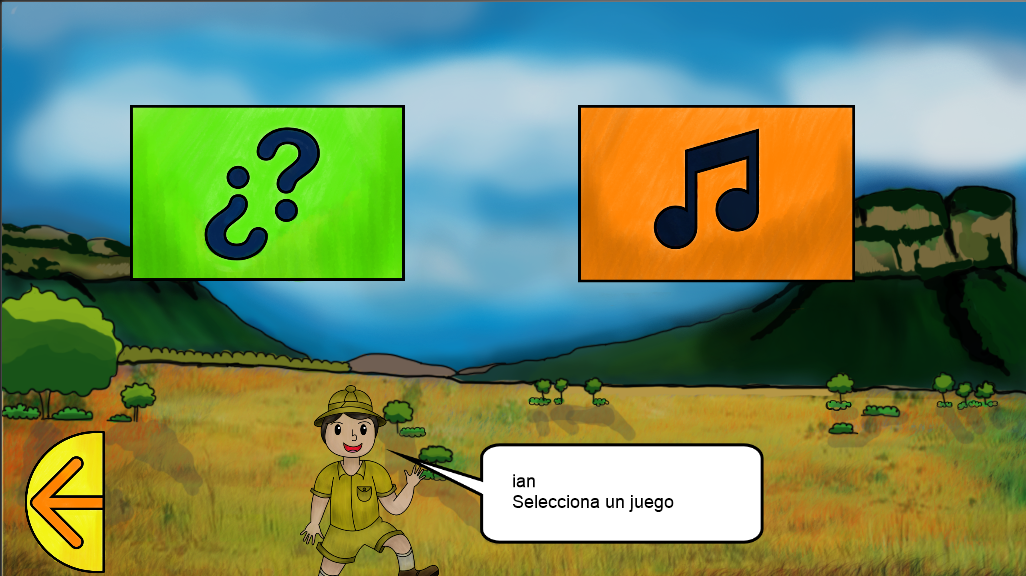
\includegraphics[width=12cm,height=6cm] {imagenes/seleccionjuego.PNG}
	\end{center}
	\caption{Selecci�n de Juegos}\label{selJue}
\end{figure}

\subsubsection{Juego 1: Adivinanzas}

El juego de las adivinanzas consiste en resolver acertijos sobre los elementos que participan en el cuento, cuento quefue seleccionado anteriormente. Para ello podr� reproducir la adivinanza y podr� usar pistas que ayuden a resolver esta adivinanza.  (Figura\ref{jueAdi}).

\begin{figure}[htf]
	\begin{center}
		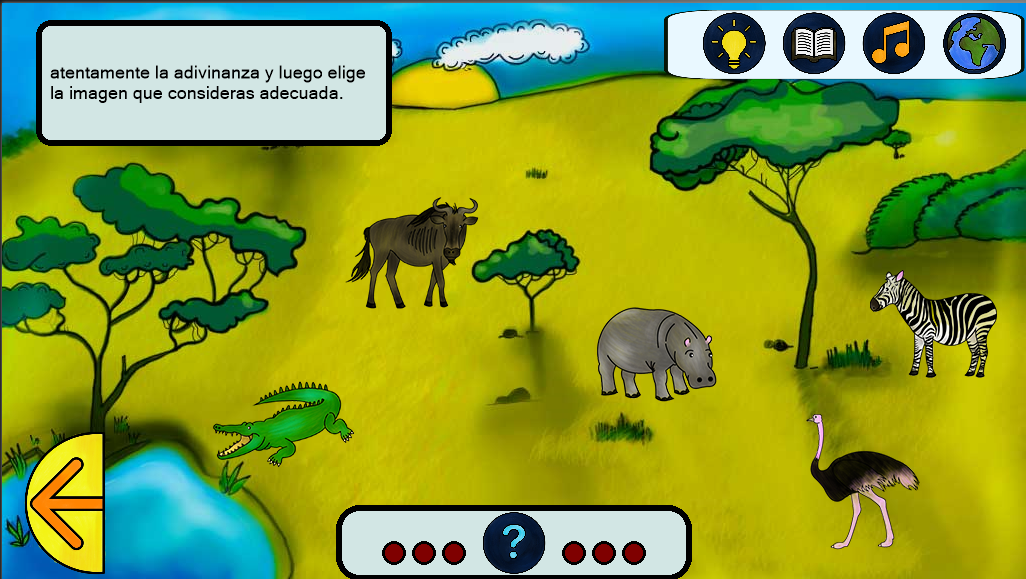
\includegraphics[width=12cm,height=6cm] {imagenes/adivinanza.PNG}
	\end{center}
	\caption{Juego 1 : Adivinanzas}\label{jueAdi}
\end{figure}

\newpage
\subsubsection{Juego 2: Pictograma Musical}

El pictograma musical consiste en completar la letra de una canci�n a trav�s de im�genes de los animales del cuento seleccionado. Al momento de completar la canci�n, se reproducir� y se dar� la posibilidad de grabar la voz acompa�ada con el instrumental de la canci�n. (Figura\ref{juePic}).

\begin{figure}[htf]
	\begin{center}
		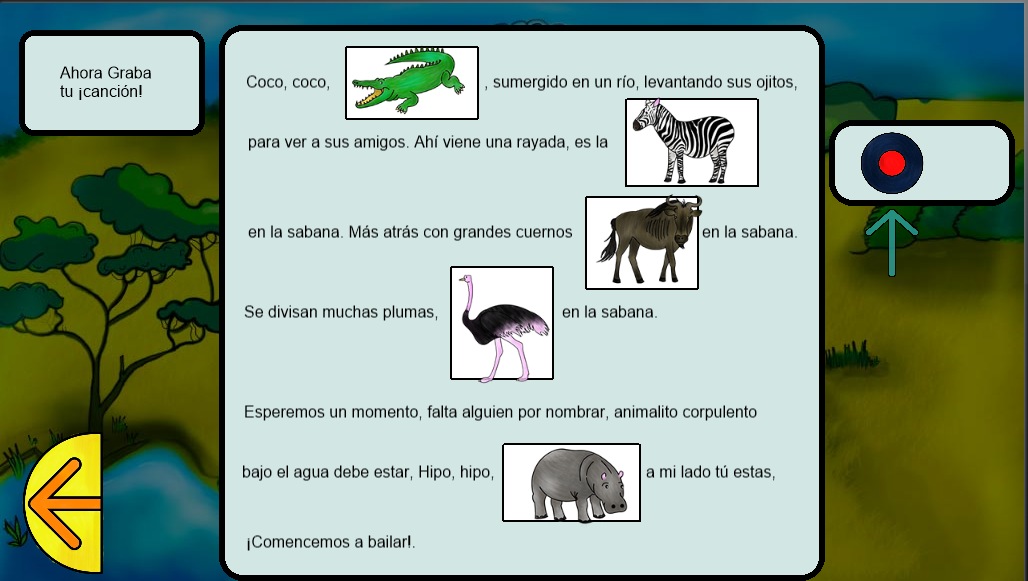
\includegraphics[width=12cm,height=6cm] {imagenes/pictograma.PNG}
	\end{center}
	\caption{Juego 2 : Pictograma Musical}\label{juePic}
\end{figure}



\chapter{Conclusi�n}
\label{conclusion}


Durante este trabajo de t�tulo se abarcaron distintas etapas que permitieron fabricar el software, tales como: el Marco referencial (Marco conceptual y Estado del arte), la etapa de Definici�n del problema y an�lisis, la etapa de Dise�o y por �ltimo la etapa de implementaci�n.\\

En la etapa de Marco referencial, se investig� sobre las dificultades del lenguaje que presentan en ni�os 3-6 a�os, comprendiendo que cada problema abarca a un nivel de lenguaje, permitiendo potenciar esos niveles atrav�s de las actividades desarrolladas en la aplicaci�n m�vil.

Adem�s se realiz� una investigaci�n sobre el estado actual de los software desarrollados para este �mbito, concluyendo que existen pocas herramientas que potencien el desarrollo del lenguaje y reflejen la realidad chilena.\\

En la etapa de Definici�n del problema y an�lisis, se estableci� los requerimientos funcionales y no funcionales, casos de usos, modelo conceptual, diagramas de estados del software implementado, estableciendo m�s concretamente la propuesta y soluci�n de este trabajo de t�tulo. Adem�s se defini� los objetivos generales y espec�ficos, alcanzados en la etapa de implementaci�n.\\

Durante la etapa de Dise�o, se defini� la arquitectura android para implementar el software, ya que en temas de costos es muy alcanzable para cualquier persona que quiera obtener de la herramienta implementada.
Tambi�n se genera los primeros prototipos de la aplicaci�n m�vil, que reflejaban como ser�an abarcadas las funcionalidades establecidas en los requerimientos.
Adem�s se establecenlos  diagrama de navegaci�n de la aplicaci�n, diagrama de clases,  diagrama de componentes, como tambi�n el dise�o de pruebas.

\clearpage
\newpage
En el dise�o de pruebas se estableci� realizar 3 etapas, siendo las pruebas unitarias, pruebas de integraci�n y las pruebas de usuarios, donde tendr�n como objetivo encontrar fallas que no fueron identificadas durante la etapa de implementaci�n.

Con respecto al dise�o de datos, se decidi� no ocupar base de datos, dado que el software no guarda datos, solamente utiliza recursos como por ejemplo: m�sica, sonidos e im�genes.\\

En la etapa de Implementaci�n se investig� un framework que ayud� a facilitar el desarrollo nativo en Android, llamado Corona SDK, el cual se basa en el lenguaje script ligero llamado Lua, de f�cil aprendizaje.

Este framework tiene soporte para el desarrollo de juegos, entregando funcionalidades que facilitan el desarrollo de las actividades establecidas para cada cuento y juego, garantizando el rendimiento y la utilizaci�n de un componente del dipositivo m�vil: El micr�fono.\\


Con la aplicaci�n terminada, se espera realizar las pruebas unitarias, integraci�n y de usuarios, dise�adas en el etapa de dise�o, como tambi�n, se almacenar� la aplicaci�n m�vil en la plataforma google play, donde podr�n descargar gratuitamente en los dispositivos m�viles. 
Estas actividades est�n planificadas para el segundo semestre del trabajo de t�tulo.












































%\include{capitulo4}
%\include{capitulo5}

%\appendix

%
\chapter{Caso de Usos Expandidos} \label{casos}

\begin{table}[h]
	
	\begin{tabular}{rp{11cm}}
		
		{\bf Id} &      CU002 \\
		
		{\bf Nombre} &  Seleccionar Personaje  \\
		
		{\bf Actor} &   Ni�o. \\
		
		{\bf Prop�sito} & El ni�o elige un personaje principal.\\
		
		{\bf Resumen} & 
		Elegir un personaje principal de los dos disponibles (Un ni�o explorador o una ni�a exploradora). \\
		
		{\bf Precondici�n} &    Ver Presentaci�n       \\
		
		{\bf Ref. Cruzadas} &  REF005, CU001.      \\
		
		& \\
	\end{tabular}
	
	\begin{tabular}{|p{7cm}|p{7cm}|}
		\hline
		\multicolumn{ 2}{|c|}{{\bf Curso Normal}} \\
		\hline
		Actor &    Sistema \\
		\hline
		1. El ni�o ingresar� su nombre. & \\
		
		& 2. El sistema guarda el nombre por la sesi�n solamente y lo muestra por pantalla. \\
		
		3. El ni�o seleccionar� el personaje "ni�o explorador" o "ni�a exploradora". & \\
		
		& 4. El sistema mostrar� la elecci�n del personaje.\\
		
		5. El ni�o presionar� boton siguiente.&\\
		
		& 6. Se prodece a confirmar la elecci�n del personaje.\\
		
		7. El ni�o confirmar la elecci�n.&\\
		
		& 8. Se prodece al siguiente caso de uso.\\ \hline
		
		
	\end{tabular}  
	
	\caption{Caso de Uso Extendido: Seleccionar Personaje.} \label{selper}
\end{table}



\begin{table}[h]
	
\begin{tabular}{|p{7cm}|p{7cm}|}\hline
\multicolumn{ 2}{|c|}{{\bf Curso Alternativo 1}} \\
\hline
7. El ni�o no confirmar la elecci�n del personaje . & \\

& 8. El sistema mostrar� nuevamente la selecci�n del personaje. \\ \hline

\multicolumn{ 2}{|c|}{{\bf Curso Alternativo 2}} \\
\hline
7. El ni�o confirma, pero falta el ingreso del nombre o la elecci�n del personaje . & \\

& 8. El sistema mostrar� nuevamente el caso de uso "Seleccionar Personaje". \\ \hline

\end{tabular} 
\caption{Caso de Uso Extendido: Seleccionar Personaje.} \label{selper}

\end{table}

\begin{table}[h]
	
	\begin{tabular}{rp{11cm}}
		
		{\bf Id} &      CU003 \\
		
		{\bf Nombre} &  Escoger Ambiente  \\
		
		{\bf Actor} &   Ni�o, educadora parvularia. \\
		
		{\bf Prop�sito} & El ni�o / educadora escoge un ambiente.\\
		
		{\bf Resumen} & 
		Seleccionar un ambiente para desarollar la historia para las actividades. \\
		
		{\bf Precondici�n} &     -       \\
		
		{\bf Ref. Cruzadas} &  REF004, REF006.      \\
		
		
		& \\
	\end{tabular}
	
	\begin{tabular}{|p{7cm}|p{7cm}|}
		\hline
		\multicolumn{ 2}{|c|}{{\bf Curso Normal}} \\
		\hline
		Actor &    Sistema \\
		\hline
		1. El ni�o / educadora seleccionar� un ambiente. & \\
		
		& 2. El sistema mostrar� el ambiente cargando im�genes y m�sica asociadas. \\
		
		3. El ni�o / educadora presionar� el bot�n siguiente para seguir la pantalla siguiente. & \\
		
		& 4. El sistema mostrar� la pantalla que asociada.\\
		
		5. El ni�o presionar� la �ltima vez el bot�n siguiente, para finalizar &\\
		
		& 6. Al momento de finalizar, se proceder� a mostrar el siguiente caso de uso.\\ \hline
		
		\multicolumn{ 2}{|c|}{{\bf Curso Alternativo 1}} \\
		\hline
		4.1 El ni�o seleccionar� el caso de uso "Escoger Herramienta". & \\
		
		& 4.2 El sistema mostrar� el caso de uso "Escoger Herramienta". \\ \hline
		
		\multicolumn{ 2}{|c|}{{\bf Curso Alternativo 2}} \\
		\hline
		1 El ni�o presionar� el bot�n volver atr�s, para volver al caso de uso "Seleccionar Personaje" CU002. & \\
		
		& 2 El sistema mostrar� el caso de uso CU002. \\ \hline
		
		
	\end{tabular}  
	
	\caption{Caso de Uso Extendido: Escoger Ambiente.}\label{escoamb}
\end{table}


\newpage
\clearpage

\begin{table}[h]
	
	\begin{tabular}{rp{11cm}}
		
		{\bf Id} &      CU004 \\
		
		{\bf Nombre} &  Escoger Cuento  \\
		
		{\bf Actor} &   Ni�o, educadora parvularia. \\
		
		{\bf Prop�sito} & El ni�o / educadora escoge un cuento.\\
		
		{\bf Resumen} & 
		Seleccionar un cuento para desarollar la historia para la actividad adivinanzas y pictograma musical. \\
		
		{\bf Precondici�n} &     Escoger Ambiente      \\
		
		{\bf Ref. Cruzadas} &  REF004, CU003.      \\
		
		& \\
	\end{tabular}
	
	\begin{tabular}{|p{7cm}|p{7cm}|}
		\hline
		\multicolumn{ 2}{|c|}{{\bf Curso Normal}} \\
		\hline
		Actor &    Sistema \\
		\hline
		1. El ni�o / educadora seleccionar� un cuento. & \\
		
		& 2. El sistema mostrar� el cuento cargando im�genes y m�sica asociadas. \\
		
		3. El ni�o / educadora presionar� el bot�n siguiente para comenzar el cuento. & \\
		
		& 4. El sistema mostrar� la pantalla asociada al cuento.\\
		
		5. El ni�o presionar� la �ltima vez el bot�n siguiente, para finalizar el cuento &\\
		
		& 6. Al momento de finalizar, se proceder� a mostrar el siguiente caso de uso.\\ \hline
		
		
		\multicolumn{ 2}{|c|}{{\bf Curso Alternativo 1}} \\
		\hline
		1. El ni�o / educadora seleccionar� el bot�n volver.  & \\
		
		& 2. El sistema volver� a la �ltima pantalla del ambiente. \\ \hline
		
		\multicolumn{ 2}{|c|}{{\bf Curso Alternativo 2}} \\
		\hline
		4.1 El ni�o seleccionar� el caso de uso "Escoger Herramienta". & \\
		
		& 4.2 El sistema mostrar� el caso de uso "Escoger Herramienta". \\ \hline
		
	\end{tabular} 
	
	\caption{Caso de Uso Extendido: Escoger Cuento.}\label{escoher}
\end{table}

\clearpage

\begin{table}[h]
	
	\begin{tabular}{rp{11cm}}
		
		{\bf Id} &      CU005 \\
		
		{\bf Nombre} &  Seleccionar Juego  \\
		
		{\bf Actor} &   Ni�o, educadora parvularia. \\
		
		{\bf Prop�sito} & El ni�o / educadora escoge un juego.\\
		
		{\bf Resumen} & 
		Seleccionar el juego de las adivinanzas o pictograma musical. \\
		
		{\bf Precondici�n} &    Escoger Cuento     \\
		
		{\bf Ref. Cruzadas} &  REF011, CU004.      \\
		
		
		& \\
	\end{tabular}
	
	\begin{tabular}{|p{7cm}|p{7cm}|}
		\hline
		\multicolumn{ 2}{|c|}{{\bf Curso Normal}} \\
		\hline
		Actor &    Sistema \\
		\hline
		1. El ni�o / educadora seleccionar� un juego. & \\
		
		& 2. El sistema mostrar� el caso de uso seg�n el juego seleccionado. \\ \hline
		
		\multicolumn{2}{|c|}{{\bf Curso Alternativo 1}} \\
		\hline
		1. El ni�o / educadora seleccionar� el bot�n volver. & \\
		
		& 2. El sistema volver� a la �ltima pantalla del caso de uso "Escoger Cuento" CU004. \\ \hline
		
		\multicolumn{ 2}{|c|}{{\bf Curso Alternativo 2}} \\
		\hline
		1. El ni�o / educadora seleccionar� el caso de uso "Escoger Herramienta". & \\
		
		& 2. El sistema mostrar� el caso de uso "Escoger Herramienta". \\ \hline
		
		
	\end{tabular}  
	
	\caption{Caso de Uso Extendido: Seleccionar Juego.}\label{seljuego}
\end{table}



\begin{table}[h]
	
	\begin{tabular}{rp{11cm}}
		
		{\bf Id} &      CU006 \\
		
		{\bf Nombre} & Jugar Adivinanzas  \\
		
		{\bf Actor} &   Ni�o. \\
		
		{\bf Prop�sito} & Acertar las adivinanzas.\\
		
		{\bf Resumen} & 
		El juego consiste en tener una imagen de fondo con varias im�genes, que una vez se escuche la adivinanza, seleccionar la imagen correcta, en el caso de que no pueda acertar a la correcta, podr� utilizar le bot�n "pista" que dar� m�s instrucciones para acertar la opci�n correcta. \\
		
		{\bf Precondici�n} &     -      \\
		
		{\bf Ref. Cruzadas} &  REF003, REF013.    \\
		
		
		& \\
	\end{tabular}
	
	\begin{tabular}{|p{7cm}|p{7cm}|}
		\hline
		\multicolumn{ 2}{|c|}{{\bf Curso Normal}} \\
		\hline
		Actor &    Sistema \\
		\hline
		1. El ni�o presionar� un bot�n para comenzar el juego. & \\
		
		& 2. El sistema cargar� las adivinanzas cargando im�genes, texto y grabaci�n de la adivinaza. \\
		
		3. El ni�o reproducir� y escuchar� la adivinanza, seleccionando la imagen correcta, para luego, seguir con la siguiente adivinanza. & \\
		
		& 4. El sistema entregar� el resultado y mostrar� la siguiente adivinanza asociada.\\
		
		5. El ni�o seleccionar� la imagen correcta de la �ltima adivinanza, para finalizar el juego.&\\
		
		& 6. Al momento de acertar la ultima adivinanza, se proceder� a mostrar el resultado  y volver� al caso de uso Seleccionar Juego CU005.\\ \hline
		
		\multicolumn{ 2}{|c|}{{\bf Curso Alternativo 1}} \\
		\hline
		2.1 El ni�o seleccionar� el caso de uso "Escoger Herramienta". & \\
		
		& 2.2 El sistema mostrar� el caso de uso "Escoger Herramienta". \\ \hline
		
		
		
	\end{tabular}  
	
	\caption{Caso de Uso Extendido: Jugar Adivinanza.}\label{jugaradi}
\end{table}

\clearpage

\begin{table}[h]
	\begin{tabular}{|p{7cm}|p{7cm}|}
		\hline
		\multicolumn{ 2}{|c|}{{\bf Curso Alternativo 2}} \\
		\hline
		2.8 Al escuchar la primera adivinanza, en el caso que el ni�o se equivoque o no entiende la adivinanza, seleccionar� el bot�n pista que ayudar� acertar. & \\
		
		& 2.9 El sistema mostrar� el caso de uso "Usar pistas". \\ \hline
	\end{tabular}
	
	\caption{Caso de Uso Extendido: Jugar Adivinanza.}
\end{table}


\begin{table}[h]
	
	\begin{tabular}{rp{11cm}}
		
		{\bf Id} &   CU007 \\
		
		{\bf Nombre} & Usar Pistas \\
		
		{\bf Actor} &   Ni�o\\
		
		{\bf Prop�sito} & Utilizar ayuda para resolver adivinanza.\\
		
		{\bf Resumen} & 
		La opci�n "pistas", entregar� descripciones adicionales para cada una de las adivinanzas, permitiendo que el ni�o pueda resolver m�s f�cil la adivinanza.\\
		
		{\bf Precondici�n} &   Jugar Adivinanzas  \\
		
		{\bf Ref. Cruzadas} &  REF003, REF013, CU006. \\
		
		
		& \\
	\end{tabular}
	
\end{table}

\begin{table}[h]
	\begin{tabular}{|p{7cm}|p{7cm}|}\hline
		
		\multicolumn{ 2}{|c|}{{\bf Curso Normal}} \\
		\hline
		1. El ni�o selecciona "Usar Pistas". & \\
		
		& 2. El sistema mostrar� la interfaz de "Usar Pistas". \\ 
		
		3. El ni�o selecciona reproducir nueva pista. & \\
		
		& 4. El sistema reproducir� la grabaci�n asociada a la pista de la imagen. \\
		
		5. El ni�o presiona volver a la pantalla anterior. & \\
		
		& 6. El sistema redireccionar� al caso de uso "Jugar Adivinanzas", donde fue invocado. \\ \hline
		
		\multicolumn{ 2}{|c|}{{\bf Curso Alternativo 1}} \\
		\hline
		3. El ni�o selecciona volver a la pantalla anterior. & \\
		
		& 4. El sistema redireccionar� al caso de uso "Jugar Adivinanzas", donde fue invocado. \\ \hline	
		
		\multicolumn{ 2}{|c|}{{\bf Curso Alternativo 2}} \\
		\hline
		3. El ni�o selecciona reiteradas veces "Nueva Pista". & \\
		
		& 4. El sistema reproducir� m�ximo 3 pistas, indicando un mensaje al ni�o de l�mite de pistas, por lo que tendr� una opci�n de pasar a la siguiente adivinanza, volviendo al caso de uso "Jugar Adivinanzas" CU006. \\ \hline	
		
		
	\end{tabular}  
	
	\caption{Caso de Uso Extendido: Usar Pistas.}\label{usarpista}
\end{table}



\newpage
\clearpage
\begin{table}[h]
	\begin{tabular}{rp{11cm}}
		
		{\bf Id} &      CU008 \\
		
		{\bf Nombre} &  Jugar Pictograma Musical  \\
		
		{\bf Actor} &   Ni�o. \\
		
		{\bf Prop�sito} & Completar Canciones.\\
		
		{\bf Resumen} & 
		El ni�o a trav�s de canciones completar� la letra de la canci�n arrastrando im�genes. \\
		
		{\bf Precondici�n} &  Seleccionar Juego \\
		
		{\bf Ref. Cruzadas} &  REF012, REF003, CU005.      \\
		
		
		& \\
	\end{tabular}
	
	\begin{tabular}{|p{7cm}|p{7cm}|}
		\hline
		\multicolumn{ 2}{|c|}{{\bf Curso Normal}} \\
		\hline
		Actor &    Sistema \\
		\hline
		1. El ni�o seleccionar� el juego pictograma musical. & \\
		
		& 2. El sistema mostrar� la interfaz del pictograma musical, cargando im�genes, texto y canciones. \\
		
		3. El ni�o escuchar� la canci�n, moviendo la imagen correcta en la oraci�n. & \\
		
		& 4. El sistema entregar� por pantalla el resultado, esperando la siguiente respuesta.\\
		
		5. El ni�o mover� la �ltima imagen correcta para finalizar el juego.&\\
		
		& 6. Al momento de finalizar, se proceder� a mostrar el resultado y volver� al caso de uso Seleccionar Juego CU005 .\\ \hline
		
		\multicolumn{ 2}{|c|}{{\bf Curso Alternativo 1}} \\
		\hline
		4.1 El ni�o seleccionar� el caso de uso "Escoger Herramienta". & \\
		
		& 4.2 El sistema mostrar� el caso de uso "Escoger Herramienta". \\ \hline
		
		
		
	\end{tabular}  
	
	\caption{Caso de Uso Extendido: Jugar Pictograma Musical.} \label{jugarpicto}
\end{table}

\clearpage
\newpage

\begin{table}[h]
	\begin{tabular}{|p{7cm}|p{7cm}|}\hline
		
		\multicolumn{ 2}{|c|}{{\bf Curso Alternativo 2}} \\
		\hline
		2.6 El ni�o se equivoca de imagen. & \\
		
		& 2.7 El sistema mostrar� el resultado, negando que la imagen quede en la oraci�n (efecto de rebote al utilizar el drag and drop). \\ 
		
		2.8 El ni�o podr� reproducir nuevamente la canci�n pulsando un bot�n de m�sica. & \\
		
		& 2.9 El sistema entregar� la canci�n a escuchar. \\ \hline
		
		\multicolumn{ 2}{|c|}{{\bf Curso Alternativo 3}} \\
		\hline
		1. � 4.1 El ni�o presiona el bot�n volver. & \\
		
		& 2. � 4.2 El sistema mostrar� el caso de uso "Seleccionar Juego". \\ \hline
		
	\end{tabular}  
	
	\caption{Caso de Uso Extendido: Jugar Pictograma Musical.}
\end{table}

\clearpage
\begin{table}[h]
	
	\begin{tabular}{rp{11cm}}
		
		{\bf Id} &      CU009 \\
		
		{\bf Nombre} &  Escoger Herramientas  \\
		
		{\bf Actor} &   Ni�o. \\
		
		{\bf Prop�sito} & Escoger una herramienta que proporcione una funcionalidad en la aplicaci�n.\\
		
		{\bf Resumen} & 
		Seleccionar la funcionalidad de activar/desactivar la musica de la pantalla, mostrar el diccionario con un bot�n de una lupa y un bot�n del planeta tierra para volver al men� principal de la aplicaci�n. \\
		
		{\bf Precondici�n} &     -       \\
		
		{\bf Ref. Cruzadas} &  REF001, REF002, REF009, REF014, REF010.      \\
		
		
		& \\
	\end{tabular}
	
	\begin{tabular}{|p{7cm}|p{7cm}|}
		\hline
		\multicolumn{ 2}{|c|}{{\bf Curso Normal}} \\
		\hline
		Actor &    Sistema \\
		\hline
		1. El ni�o / educadora selecciona un boton del conjunto de funcionalidades. & \\
		
		& 2. El sistema mostrar� la funcionalidad seleccionada. \\ \hline
		
	\end{tabular}  
	
	\caption{Caso de Uso Extendido: Escoger Herramientas.} \label{escoherra}
\end{table}

\clearpage
\begin{table}[h]
	
	\begin{tabular}{rp{11cm}}
		
		{\bf Id} &      CU010 \\
		
		{\bf Nombre} &  Ver Diccionario  \\
		
		{\bf Actor} &   Ni�o. \\
		
		{\bf Prop�sito} & Entregar vocabulario nuevo, para el entendimiento de las palabras e im�genes usadas.\\
		
		{\bf Resumen} & 
		Seleccionar la funcionalidad de mostrar un diccionario que contendr� el significado de las palabras e identificaci�n de im�genes o pictogramas. \\
		
		{\bf Precondici�n} &  Escoger Herramientas \\
		
		{\bf Ref. Cruzadas} & REF009, REF010, CU009.     \\
		
		
		& \\
	\end{tabular}
	
	\begin{tabular}{|p{7cm}|p{7cm}|}
		\hline
		\multicolumn{ 2}{|c|}{{\bf Curso Normal}} \\
		\hline
		Actor &    Sistema \\
		\hline
		1. El ni�o / educadora escoge el boton lupa. & \\
		
		& 2. El sistema mostrar� la interfaz del diccionario . \\
		
		3. El ni�o / educadora presionar� la imagen o palabra disponible en el diccionario. & \\
		
		& 4. El sistema mostrar� interfaz del elemento  seleccionado del diccionario, entregando sonido, imagen y texto.\\
		
		5. El ni�o presionar� finalizar diccionario.  &\\
		
		& 6. El sistema redireccionar a la pantalla Escoger Herramientas CU003.\\ \hline
		
		\multicolumn{ 2}{|c|}{{\bf Curso Alternativo}} \\
		\hline
		
		1. El ni�o / educadora  escoge finalizar diccionario o el bot�n volver, regresando a la pantalla anterior. & \\
		
		& 2. El sistema proceder� volver al caso de uso donde fue llamado "Escoger Herramientas", CU003.\\ \hline
		
		
	\end{tabular}  
	
	\caption{Caso de Uso Extendido: Ver Diccionario.}\label{verdic}
\end{table}

\clearpage
\begin{table}[h]
	
	\begin{tabular}{rp{11cm}}
		
		{\bf Id} &      CU011 \\
		
		{\bf Nombre} &  Grabar Voz \\
		
		{\bf Actor} &   Ni�o. \\
		
		{\bf Prop�sito} & Grabar la voz del ni�o, permitiendo desarrollar la consciencia fonol�gica.\\
		
		{\bf Resumen} & 
		La funcionalidad grabar voz, permite que el ni�o escuche las palabras o frases que dice, en el transcurso de la aplicaci�n, creando interacci�n entre la aplicaci�n y el ni�o. \\
		
		{\bf Precondici�n} &  Escoger Herramientas \\
		
		{\bf Ref. Cruzadas} &  REF001, CU009.      \\
		
		
		& \\
	\end{tabular}
	
	\begin{tabular}{|p{7cm}|p{7cm}|}
		\hline
		\multicolumn{ 2}{|c|}{{\bf Curso Normal}} \\
		\hline
		Actor &    Sistema \\
		\hline
		1. El ni�o escoge el bot�n de un micr�fono. & \\
		
		& 2. El sistema mostrar� un mensaje que se encuentra grabando la voz .\\
		
		3. El ni�o presionar� nuevamente el bot�n del micr�fono para inicializar la grabaci�n & \\
		
		& 4. El sistema mostrar� un mensaje que la grabaci�n ha comenzado.\\
		
		5. El ni�o presionar� nuevamente el bot�n del micr�fono para finalizar la grabaci�n.  &\\
		
		& 6. El sistema mostrar� un mensaje que la grabaci�n ha finalizado.\\ 
		
		7. El ni�o presionar� nuevamente el bot�n de reproducir la grabaci�n. &\\
		
		& 8. El sistema reproducir� la grabaci�n.\\ 
		
		9. El ni�o presionar� finalizar. &\\
		
		& 10. El sistema volver� a la pantalla anterior.\\ \hline
		
		
		
		
		
		\multicolumn{ 2}{|c|}{{\bf Curso Alternativo}} \\
		\hline
		
		3. El ni�o no pulsa el bot�n del micr�fono nuevamente para finalizar la grabaci�n. & \\
		
		& 4. El sistema proceder� a finalizar dentro de 50 segundos la grabaci�n, mostrando el mensaje finalizaci�n de la grabaci�n.\\ \hline
		
		
	\end{tabular}  
	
	\caption{Caso de Uso Extendido: Grabar Voz.}\label{grabarvoz}
\end{table}

\clearpage
\begin{table}[h]
	
	\begin{tabular}{rp{11cm}}
		
		{\bf Id} &      CU012 \\
		
		{\bf Nombre} &  Regresar Ambientes \\
		
		{\bf Actor} &   Ni�o. \\
		
		{\bf Prop�sito} & Volver a la pantalla principal de selecci�n de ambientes.\\
		
		{\bf Resumen} & 
		Entregar la posibilidad de volver al men� de elecci�n de ambiente durante las actividades. \\
		
		{\bf Precondici�n} &  Escoger Herramientas \\
		
		{\bf Ref. Cruzadas} &  REF014, CU009.      \\
		
		
		& \\
	\end{tabular}
	
	\begin{tabular}{|p{7cm}|p{7cm}|}
		\hline
		\multicolumn{ 2}{|c|}{{\bf Curso Normal}} \\
		\hline
		Actor &    Sistema \\
		\hline
		1. El ni�o selecciona el �cono del planeta tierra. & \\
		
		& 2. El sistema enviar� un mensaje de confirmaci�n .\\
		
		3. El ni�o confirmar� volver a la selecci�n de ambiente. & \\
		
		& 4. El sistema redireccionar� al caso de uso "Escoger Ambiente".\\ \hline
		
		
		\multicolumn{ 2}{|c|}{{\bf Curso Alternativo}} \\
		\hline
		
		3. El ni�o negar� volver a la selecci�n de ambientes.& \\
		
		& 4. El sistema volver� a la pantalla donde fue llamado.\\ \hline
		
	\end{tabular}  
	
	\caption{Caso de Uso Extendido: Regresar Ambientes.}\label{regamb}
\end{table}	


\chapter{Diagramas de Secuencias} \label{diagrama}

\begin{figure}[htf]
	\begin{center}
		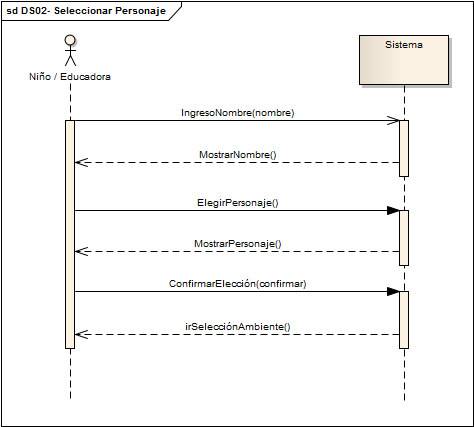
\includegraphics[width=10cm,height=8cm] {imagenes/DS02.png}
	\end{center}
	\caption{Caso de uso: Seleccionar Personaje}
\end{figure}

\begin{figure}[htf]
	\begin{center}
		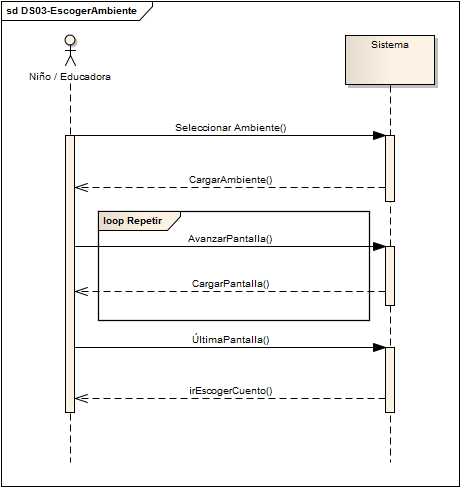
\includegraphics[width=10cm,height=8cm] {imagenes/DS03.png}
	\end{center}
	\caption{Caso de uso: Escoger Ambiente}
\end{figure}

\begin{figure}[htf]
	\begin{center}
		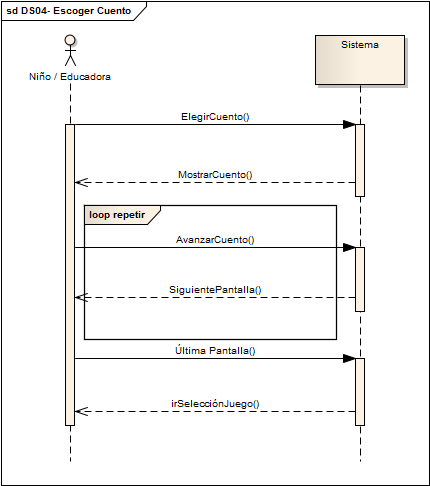
\includegraphics[width=10cm,height=8cm] {imagenes/DS04.png}
	\end{center}
	\caption{Caso de uso: Escoger Cuento}
\end{figure}

\begin{figure}[htf]
	\begin{center}
		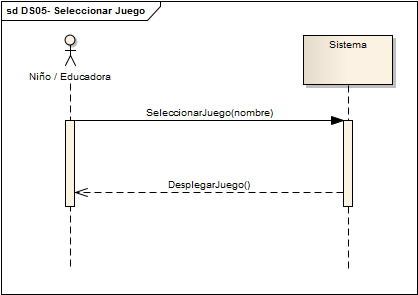
\includegraphics[width=10cm,height=8cm] {imagenes/DS05.png}
	\end{center}
	\caption{Caso de uso: Seleccionar Juego}
\end{figure}

\begin{figure}[htf]
	\begin{center}
		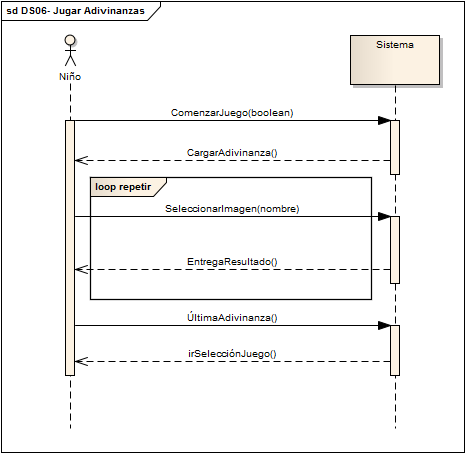
\includegraphics[width=10cm,height=8cm] {imagenes/DS06.png}
	\end{center}
	\caption{Caso de uso: Jugar Adivinanza}
\end{figure}

\begin{figure}[htf]
	\begin{center}
		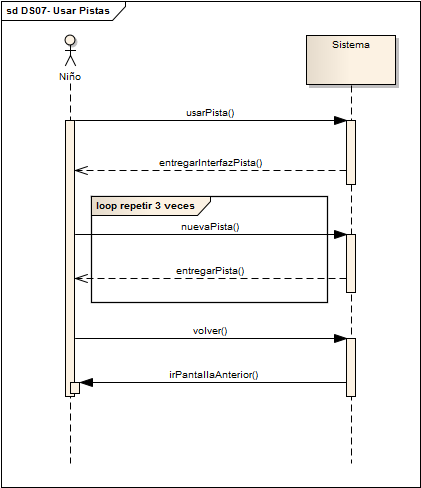
\includegraphics[width=10cm,height=8cm] {imagenes/DS07.png}
	\end{center}
	\caption{Caso de uso: Usar Pistas}
\end{figure}

\begin{figure}[htf]
	\begin{center}
		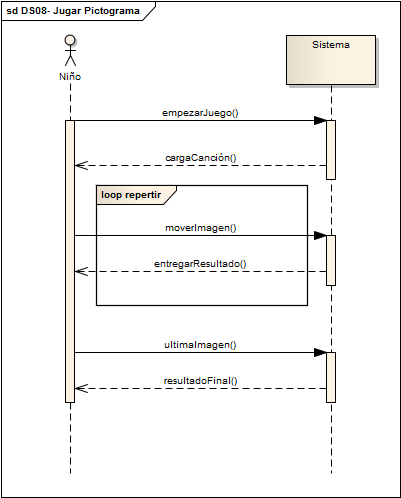
\includegraphics[width=10cm,height=8cm] {imagenes/DS08.png}
	\end{center}
	\caption{Caso de uso: Jugar Pictograma}
\end{figure}

\begin{figure}[htf]
	\begin{center}
		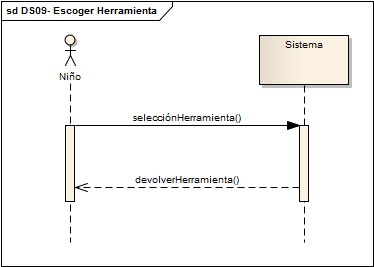
\includegraphics[width=10cm,height=8cm] {imagenes/DS09.png}
	\end{center}
	\caption{Caso de uso: Escoger Herramientas}
\end{figure}


\begin{figure}[htf]
	\begin{center}
		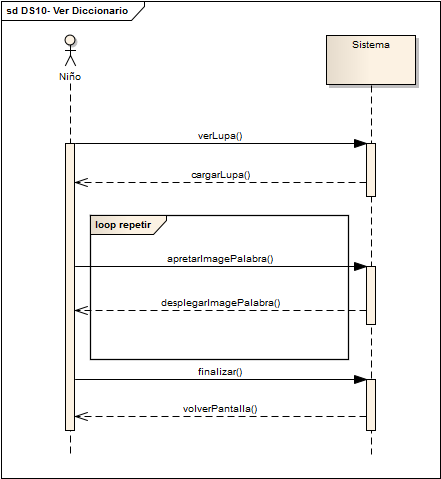
\includegraphics[width=10cm,height=8cm] {imagenes/DS10.png}
	\end{center}
	\caption{Caso de uso: Ver Diccionario}
\end{figure}

\begin{figure}[htf]
	\begin{center}
		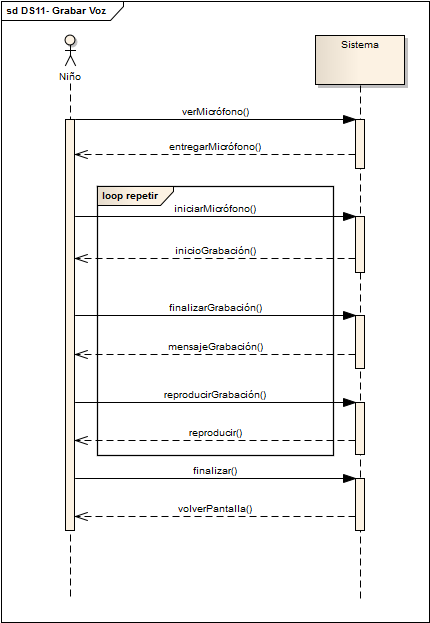
\includegraphics[width=10cm,height=8cm] {imagenes/DS11.png}
	\end{center}
	\caption{Caso de uso: Grabar Voz}
\end{figure}

\clearpage
\begin{figure}[htf]
	\begin{center}
		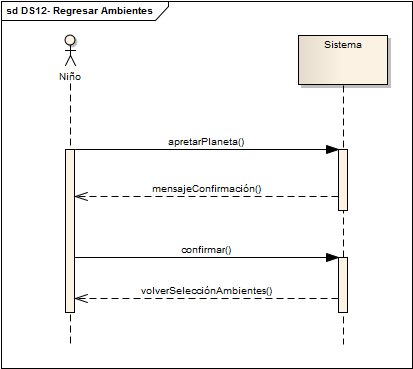
\includegraphics[width=10cm,height=8cm] {imagenes/DS12.png}
	\end{center}
	\caption{Caso de uso: Regresar Ambientes}
\end{figure}



\chapter{Diagramas de Estados} \label{estados}

\begin{figure}[htf]
	\begin{center}
		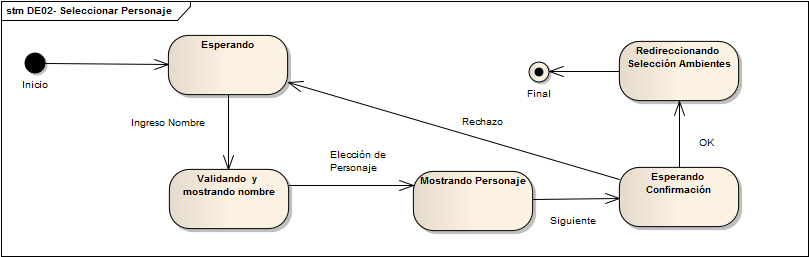
\includegraphics[width=13cm,height=6cm] {imagenes/DE02.png}
	\end{center}
	\caption{Caso de uso: Seleccionar Personaje}
\end{figure}

\begin{figure}[htf]
	\begin{center}
		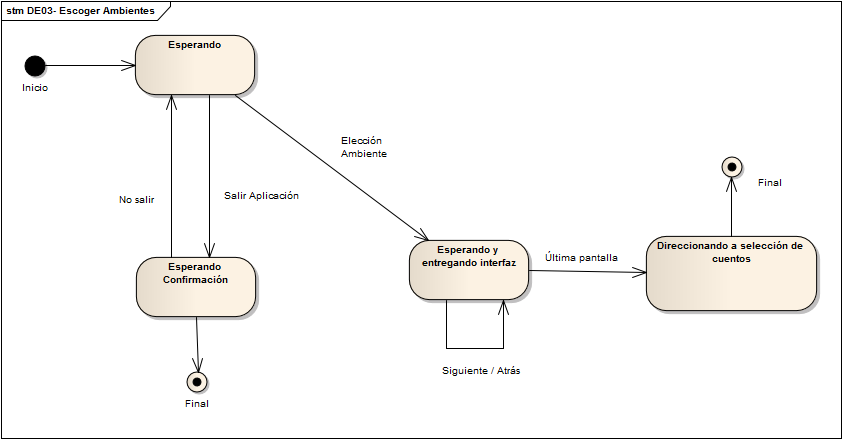
\includegraphics[width=13cm,height=6cm] {imagenes/DE03.png}
	\end{center}
	\caption{Caso de uso: Escoger Ambiente}
\end{figure}

\begin{figure}[htf]
	\begin{center}
		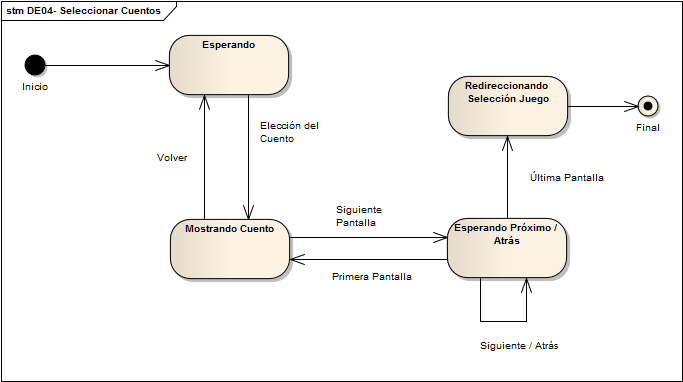
\includegraphics[width=13cm,height=6cm] {imagenes/DE04.png}
	\end{center}
	\caption{Caso de uso: Escoger Cuento}
\end{figure}

\begin{figure}[htf]
	\begin{center}
		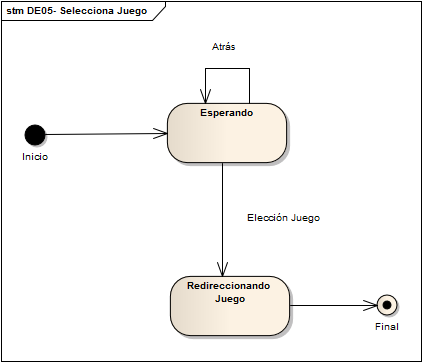
\includegraphics[width=13cm,height=6cm] {imagenes/DE05.png}
	\end{center}
	\caption{Caso de uso: Seleccionar Juego}
\end{figure}

\begin{figure}[htf]
	\begin{center}
		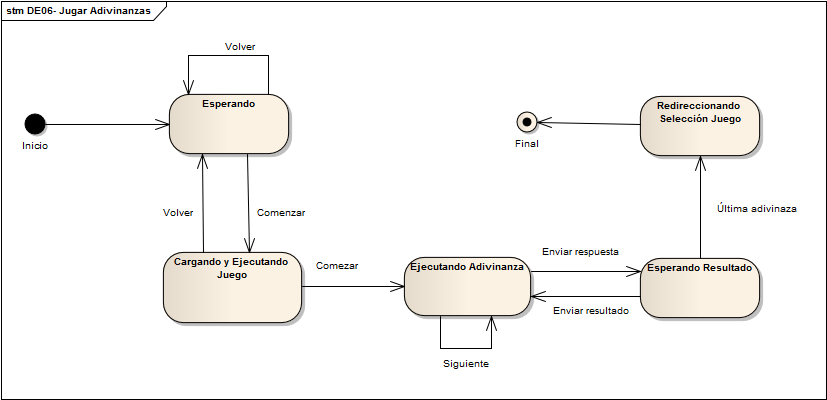
\includegraphics[width=13cm,height=6cm] {imagenes/DE06.png}
	\end{center}
	\caption{Caso de uso: Jugar Adivinanza}
\end{figure}

\begin{figure}[htf]
	\begin{center}
		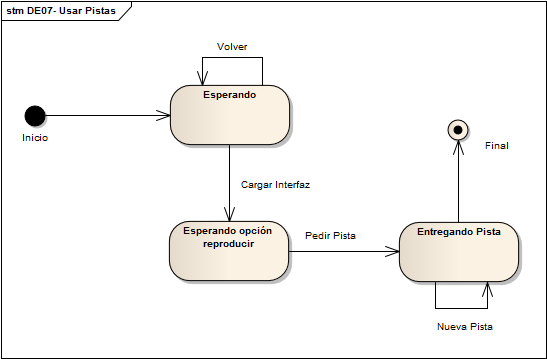
\includegraphics[width=13cm,height=6cm] {imagenes/DE07.png}
	\end{center}
	\caption{Caso de uso: Usar Pistas}
\end{figure}

\begin{figure}[htf]
	\begin{center}
		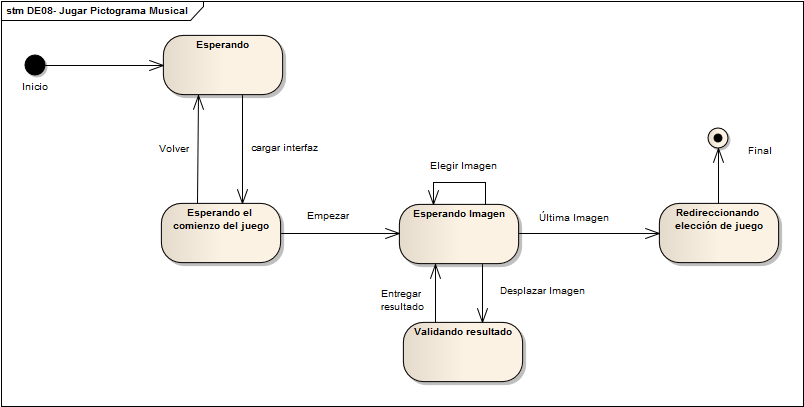
\includegraphics[width=13cm,height=6cm] {imagenes/DE08.png}
	\end{center}
	\caption{Caso de uso: Jugar Pictograma}
\end{figure}

\begin{figure}[htf]
	\begin{center}
		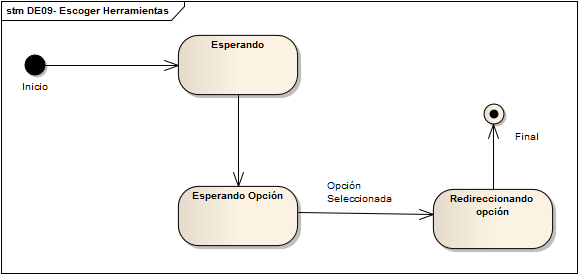
\includegraphics[width=13cm,height=6cm] {imagenes/DE09.png}
	\end{center}
	\caption{Caso de uso: Escoger Herramientas}
\end{figure}

\begin{figure}[htf]
	\begin{center}
		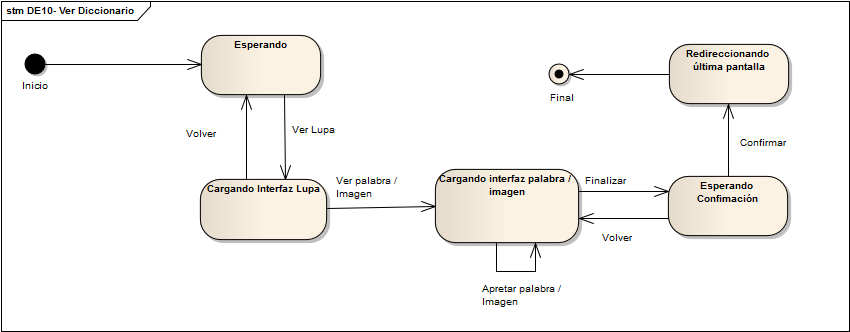
\includegraphics[width=13cm,height=6cm] {imagenes/DE10.png}
	\end{center}
	\caption{Caso de uso: Ver Diccionario}
\end{figure}

\begin{figure}[htf]
	\begin{center}
		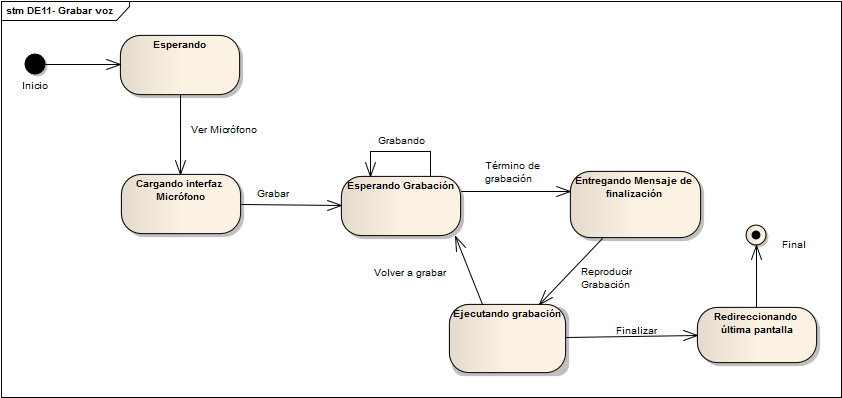
\includegraphics[width=13cm,height=6cm] {imagenes/DE11.png}
	\end{center}
	\caption{Caso de uso: Grabar Voz}
\end{figure}

\begin{figure}[htf]
	\begin{center}
		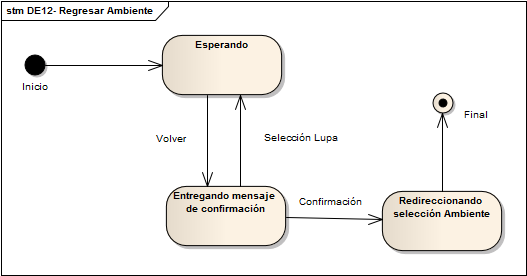
\includegraphics[width=13cm,height=6cm] {imagenes/DE12.png}
	\end{center}
	\caption{Caso de uso: Regresar Ambientes}
\end{figure}


\chapter{Dise�o de Interfaz} \label{interfaz}

\subsubsection{Prototipo 2: Pantalla de selecci�n de Personaje }

En la segunda pantalla de la aplicaci�n (Figura \ref{prot2}), el ni�o podr� ingresar su nombre y seleccionar� un personaje que participar� en la historia del cuento. El personaje seleccionado puede ser un ni�o explorador o una ni�a exploradora.\\

\begin{figure}[htf]
	\begin{center}
		\includegraphics[width=9cm,height=5cm] {imagenes/pro2.png}
	\end{center}
	\caption{Prototipo 2, Pantalla de selecci�n de personaje} \label{prot2}
\end{figure}

\newpage
\begin{table}[htf]
	
	\begin{tabular}{rp{11cm}}
		
		{\bf Id} &      CU002 \\
		
		{\bf Nombre} &  Seleccionar Personaje  \\
		
		{\bf Actor} &   Ni�o. \\
		
		{\bf Prop�sito} & El ni�o elige un personaje principal.\\
		
		{\bf Resumen} & 
		Elegir un personaje principal de los dos disponibles (Un ni�o explorador o una ni�a exploradora). \\
		
		{\bf Precondici�n} &    Ver Presentaci�n       \\
		
		{\bf Ref. Cruzadas} &  REF005, CU001.      \\
		
		& \\
	\end{tabular}
	
	\begin{tabular}{|p{7cm}|p{7cm}|}
		\hline
		\multicolumn{ 2}{|c|}{{\bf Curso Normal}} \\
		\hline
		Actor &    Sistema \\
		\hline
		1. El ni�o ingresar� su nombre [\textbf{Punto A}, Figura \ref{prot2}]. & \\
		
		& 2. El sistema guarda el nombre por la sesi�n solamente y lo muestra por pantalla. \\
		
		3. El ni�o seleccionar� el personaje "ni�o explorador" o "ni�a exploradora" [\textbf{Punto B}, Figura \ref{prot2}]. & \\
		
		& 4. El sistema mostrar� la elecci�n del personaje.\\
		
		5. El ni�o presionar� boton siguiente [\textbf{Punto C}. Figura \ref{prot2}].&\\
		
		& 6. Se prodece a confirmar la elecci�n del personaje.\\
		
		7. El ni�o confirmar la elecci�n.&\\
		
		& 8. Se prodece al siguiente caso de uso.\\ \hline
		
	\end{tabular}  
	
	\caption{Caso de Uso Extendido: Seleccionar Personaje.}
\end{table}


\newpage
\clearpage
\subsubsection{Prototipo 3: Pantalla principal, selecci�n de ambientes}

En la tercera pantalla de la aplicaci�n (Figura \ref{prot3.1} y Figura \ref{prot3.2}), se introducir� un video o animaci�n que explicar� los ambientes disponibles, siendo la sabana y el oc�ano/ant�rtida.\\

\begin{table}[h]
	
	\begin{tabular}{rp{11cm}}
		
		{\bf Id} &      CU003 \\
		
		{\bf Nombre} &  Escoger Ambiente  \\
		
		{\bf Actor} &   Ni�o, educadora parvularia. \\
		
		{\bf Prop�sito} & El ni�o / educadora escoge un ambiente.\\
		
		{\bf Resumen} & 
		Seleccionar un ambiente para desarollar la historia para las actividades. \\
		
		{\bf Precondici�n} &     -       \\
		
		{\bf Ref. Cruzadas} &  REF004, REF006.      \\
		
		
		& \\
	\end{tabular}
	
	\begin{tabular}{|p{7cm}|p{7cm}|}
		\hline
		\multicolumn{ 2}{|c|}{{\bf Curso Normal}} \\
		\hline
		Actor &    Sistema \\
		\hline
		1. El ni�o / educadora seleccionar� un ambiente [\textbf{Punto A}, Figura \ref{prot3.1}]. & \\
		
		& 2. El sistema mostrar� el ambiente cargando im�genes y m�sica asociadas. \\
		
		3. El ni�o / educadora presionar� el bot�n siguiente para seguir la pantalla siguiente [\textbf{Punto B}, Figura \ref{prot3.2}]. & \\
		
		& 4. El sistema mostrar� la pantalla que asociada.\\
		
		5. El ni�o presionar� la �ltima vez el bot�n siguiente, para finalizar &\\
		
		& 6. Al momento de finalizar, se proceder� a mostrar el siguiente caso de uso.\\ \hline
		
	\end{tabular}  
	
	\caption{Caso de Uso Extendido: Escoger Ambiente.}
\end{table}


\begin{figure}[h]
	\begin{center}
		\includegraphics[width=9cm,height=5cm] {imagenes/pro31.png}
	\end{center}
	\caption{Prototipo 3.1, Pantalla principal, selecci�n de ambientes}\label{prot3.1}
\end{figure}


\begin{figure}[h]
	\begin{center}
		\includegraphics[width=9cm,height=5cm] {imagenes/pro32.png}
	\end{center}
	\caption{Prototipo 3.2, Pantalla principal, selecci�n de ambientes}\label{prot3.2}
\end{figure}

\clearpage
\newpage
\subsubsection{Prototipo 4: Pantalla de presentaci�n de herramientas}

En la cuarta pantalla de la aplicaci�n (Figura \ref{prot4} ), previamente elegido un ambiente, se proceder� a a explicar las herramientas en la esquina superior, encontrando las siguientes:\\


\begin{itemize}
	
	\item El �cono de la cara del explorador tendr� como funcionalidad de ayudar en las pistas del juego de las adivinanzas. 
	
	\item La doble corchea tendr� la funcionar de habilitar y deshabilitar la m�sica de fondo de la aplicaci�n.
	
	\item El �cono del mundo al presionarlo volver� a la pantalla principal de selecci�n de ambientes.
	
	\item El �cono de la lupa mostrar� el diccionario asociado a la pantalla, encontrando el significado de palabras con su sonido respectivo.\\
	
\end{itemize}

\begin{table}[h]
	
	\begin{tabular}{rp{11cm}}
		
		{\bf Id} &      CU009 \\
		
		{\bf Nombre} &  Escoger Herramientas  \\
		
		{\bf Actor} &   Ni�o. \\
		
		{\bf Prop�sito} & Escoger una herramienta que proporcione una funcionalidad en la aplicaci�n.\\
		
		{\bf Resumen} & 
		Seleccionar la funcionalidad de activar/desactivar la musica de la pantalla, explorador que ayude en las pistas de la adivinanza, mostrar el diccionario con un bot�n de una lupa y un bot�n del planeta tierra para volver al men� principal de la aplicaci�n. \\
		
		{\bf Precondici�n} &     -       \\
		
		{\bf Ref. Cruzadas} &  REF001, REF002, REF009, REF014, REF010.      \\
		
		
		& \\
	\end{tabular}
	
	\begin{tabular}{|p{6cm}|p{7cm}|}
		\hline
		\multicolumn{ 2}{|c|}{{\bf Curso Normal}} \\
		\hline
		Actor &    Sistema \\
		\hline
		1. El ni�o / educadora selecciona un boton del conjunto de funcionalidades [\textbf{Punto A}, Figura \label{proto4}]. & \\
		
		& 2. El sistema mostrar� la funcionalidad seleccionada. \\ \hline
		
	\end{tabular}  
	
	\caption{Caso de Uso Extendido: Escoger Herramientas.}
\end{table}


\newpage
\clearpage
\begin{figure}[htf]
	\begin{center}
		\includegraphics[width=9cm,height=5cm] {imagenes/pro4.png}
	\end{center}
	\caption{Prototipo 4, Pantalla de presentaci�n de herramientas} \label{prot4}
\end{figure}


\subsubsection{Prototipo 5: Pantalla de selecci�n de cuentos}

En esta pantalla (Figura \ref{prot5.1}), se dar� a elegir dos cuentos que usar�n la tem�tica del ambiente elegido.\\

\begin{table}[h]
	
	\begin{tabular}{rp{11cm}}
		
		{\bf Id} &      CU004 \\
		
		{\bf Nombre} &  Escoger Cuento  \\
		
		{\bf Actor} &   Ni�o, educadora parvularia. \\
		
		{\bf Prop�sito} & El ni�o / educadora escoge un cuento.\\
		
		{\bf Resumen} & 
		Seleccionar un cuento para desarollar la historia para la actividad adivinanzas y pictograma musical. \\
		
		{\bf Precondici�n} &     Escoger Ambiente      \\
		
		{\bf Ref. Cruzadas} &  REF004, CU003.      \\
		
		& \\
	\end{tabular}
	
	\begin{tabular}{|p{7cm}|p{7cm}|}
		\hline
		\multicolumn{ 2}{|c|}{{\bf Curso Normal}} \\
		\hline
		Actor &    Sistema \\
		\hline
		1. El ni�o / educadora seleccionar� un cuento [\textbf{Punto A}, Figura \ref{prot5.1}]. & \\
		
		& 2. El sistema mostrar� el cuento cargando im�genes y m�sica asociadas. \\
		
		3. El ni�o / educadora presionar� el bot�n siguiente para comenzar el cuento. & \\
		
		& 4. El sistema mostrar� la pantalla asociada al cuento.\\
		
		5. El ni�o presionar� la �ltima vez el bot�n siguiente, para finalizar el cuento [\textbf{Punto B}, Figura \ref{prot5.2}]. &\\
		
		& 6. Al momento de finalizar, se proceder� a mostrar el siguiente caso de uso.\\ \hline
		
	\end{tabular} 
	
	\caption{Caso de Uso Extendido: Escoger Cuento.}
\end{table}



\begin{figure}[htf]
	\begin{center}
		\includegraphics[width=9cm,height=5cm] {imagenes/pro51.png}
	\end{center}
	\caption{Prototipo 5.1, Pantalla de selecci�n de cuentos} \label{prot5.1}
\end{figure}


\begin{figure}[htf]
	\begin{center}
		\includegraphics[width=9cm,height=5cm] {imagenes/pro52.png}
	\end{center}
	\caption{Prototipo 5.2, Pantalla de la historia de cuentos} \label{prot5.2}
\end{figure}


\newpage
\clearpage
\subsubsection{Prototipo 6: Pantalla de la selecci�n de actividades}

En esta pantalla el ni�o podr� elegir que actividad realizar, encontrando el juego de las adivinanzas y el pictograma musical.
Al seleccionar uno de ellos, se cargar� cada juego en una pantalla nueva.\\

\begin{table}[h]
	
	\begin{tabular}{rp{11cm}}
		
		{\bf Id} &      CU005 \\
		
		{\bf Nombre} &  Seleccionar Juego  \\
		
		{\bf Actor} &   Ni�o, educadora parvularia. \\
		
		{\bf Prop�sito} & El ni�o / educadora escoge un juego.\\
		
		{\bf Resumen} & 
		Seleccionar el juego de las adivinanzas o pictograma musical. \\
		
		{\bf Precondici�n} &    Escoger Cuento     \\
		
		{\bf Ref. Cruzadas} &  REF011, CU004.      \\
		
		
		& \\
	\end{tabular}
	
	\begin{tabular}{|p{7cm}|p{7cm}|}
		\hline
		\multicolumn{ 2}{|c|}{{\bf Curso Normal}} \\
		\hline
		Actor &    Sistema \\
		\hline
		1. El ni�o / educadora seleccionar� un juego [\textbf{Punto A}, Figura \ref{proto6} ]. & \\
		
		& 2. El sistema mostrar� el caso de uso seg�n el juego seleccionado. \\ \hline
		
	\end{tabular}  
	\caption{Caso de Uso Extendido: Seleccionar Juego.}
\end{table}


\begin{figure}[htf]
	\begin{center}
		\includegraphics[width=9cm,height=5cm] {imagenes/pro6.png}
	\end{center}
	\caption{Prototipo 6, Pantalla de la selecci�n de las actividades} \label{proto6}
\end{figure}


\clearpage
\newpage
\subsubsection{Prototipo 7: Pantalla del juego de las adivinanzas}

En esta pantalla el ni�o podr� escuchar las diferentes adivinanzas, en donde tendr� que seleccionar el dibujo que corresponda a la descripci�n nombrada. Adem�s constar� del bot�n explorador habilitado para la utilizaci�n de pistas y el bot�n del signo interrogaci�n que podr� repetir nuevamente la adivinanza. Tambi�n podr� utilizar la barra de herramientas de la parte superior derecha de la aplicaci�n.\\


\begin{figure}[h]
	\begin{center}
		\includegraphics[width=9cm,height=5cm] {imagenes/pro7.png}
	\end{center}
	\caption{Prototipo 7, Pantalla del juego de las adivinanzas}\label{proto7}
\end{figure}


\begin{table}[htf]
	
	\begin{tabular}{rp{11cm}}
		
		{\bf Id} &      CU006 \\
		
		{\bf Nombre} & Jugar Adivinanzas  \\
		
		{\bf Actor} &   Ni�o. \\
		
		{\bf Prop�sito} & Acertar las adivinanzas.\\
		
		{\bf Resumen} & 
		El juego consiste en tener una imagen de fondo con varias im�genes, que una vez se escuche la adivinanza, seleccionar la imagen correcta, en el caso de que no pueda acertar a la correcta, podr� utilizar le bot�n "pista" que dar� m�s instrucciones para acertar la opci�n correcta. \\
		
		{\bf Precondici�n} &     -      \\
		
		{\bf Ref. Cruzadas} &  REF003, REF013.    \\
		
		
		& \\
	\end{tabular}
	
	\begin{tabular}{|p{7cm}|p{7cm}|}
		\hline
		\multicolumn{ 2}{|c|}{{\bf Curso Normal}} \\
		\hline
		Actor &    Sistema \\
		\hline
		1. El ni�o presionar� un bot�n para comenzar el juego. & \\
		
		& 2. El sistema cargar� las adivinanzas cargando im�genes, texto y grabaci�n de la adivinaza. \\
		
		3. El ni�o reproducir� y escuchar� la adivinanza, seleccionando la imagen correcta, para luego, seguir con la siguiente adivinanza [\textbf{Punto A}, Figura \ref{proto7}]. & \\
		
		& 4. El sistema entregar� el resultado y mostrar� la siguiente adivinanza asociada.\\
		
		5. El ni�o seleccionar� la imagen correcta de la �ltima adivinanza, para finalizar el juego [\textbf{Punto B}, Figura \ref{proto7}].&\\
		
		& 6. Al momento de acertar la �ltima adivinanza, se proceder� a mostrar el resultado e iniciar� el juego del pictograma.\\ \hline
		
	\end{tabular}  
	
	\caption{Caso de Uso Extendido: Jugar Adivinanza.}
\end{table}


\clearpage
\newpage
\subsubsection{Prototipo 8: Pantalla de las pistas del juego de las adivinanzas}

En esta pantalla, el ni�o podr� acceder a las pistas que ayudar�n  a resolver la adivinanza. En ella podr� escuchar la pista sobre la adivinanza y podr� volver a la pantalla del juego.

\begin{table}[htf]
	
	\begin{tabular}{rp{11cm}}
		
		{\bf Id} &   CU007 \\
		
		{\bf Nombre} & Usar Pistas \\
		
		{\bf Actor} &   Ni�o\\
		
		{\bf Prop�sito} & Utilizar ayuda para resolver adivinanza.\\
		
		{\bf Resumen} & 
		La opci�n "pistas", entregar� descripciones adicionales para cada una de las adivinanzas, permitiendo que el ni�o pueda resolver m�s f�cil la adivinanza.\\
		
		{\bf Precondici�n} &   Jugar Adivinanzas  \\
		
		{\bf Ref. Cruzadas} &  REF003, REF013, CU006. \\
		
	\end{tabular}
	
\end{table}

\begin{table}[htf]
	\begin{tabular}{|p{7cm}|p{7cm}|}\hline
		
		\multicolumn{ 2}{|c|}{{\bf Curso Normal}} \\
		\hline
		1. El ni�o selecciona "Usar Pistas". & \\
		
		& 2. El sistema mostrar� la interfaz de "Usar Pistas". \\ 
		
		3. El ni�o selecciona reproducir nueva pista. [\textbf{Punto A}, Figura \ref{proto8}]. & \\
		
		& 4. El sistema reproducir� la grabaci�n asociada a la pista de la imagen. \\
		
		5. El ni�o presiona volver a la pantalla anterior.[\textbf{Punto B}, Figura \ref{proto8}] & \\
		
		& 6. El sistema redireccionar� al caso de uso "Jugar Adivinanzas", donde fue invocado. \\ \hline
		
		
	\end{tabular}  
	
	\caption{Caso de Uso Extendido: Usar Pistas.}
\end{table}

\clearpage
\newpage

\begin{figure}
	\begin{center}
		\includegraphics[width=9cm,height=5cm] {imagenes/pro8.png}
	\end{center}
	\caption{Prototipo 8, Pantalla del juego de las adivinanzas}\label{proto8}
\end{figure}


\subsubsection{Prototipo 9: Pantalla del juego del pictograma musical}

En esta pantalla el ni�o podr� escuchar la canci�n relacionada con el cuento y el ambiente seleccionado.\\
El pictograma musical consiste en arrastrar las im�genes a cada estrofa de la canci�n, en la cual si es correcta quedar� en la estrofa elegida. A medida que avance podr� reproducir la canci�n hasta la �ltima estrofa correcta.

Tambi�n, el ni�o podr� cantar la canci�n utilizando la pista de la canci�n del pictograma musical.\\


\begin{figure}[htf]
	\begin{center}
		\includegraphics[width=9cm,height=5cm] {imagenes/pro9.png}
	\end{center}
	\caption{Prototipo 8, Pantalla del juego del pictograma musical}\label{proto9}
\end{figure}


\clearpage
\newpage

\begin{table}[htf]
	\begin{tabular}{rp{11cm}}
		
		{\bf Id} &      CU008 \\
		
		{\bf Nombre} &  Jugar Pictograma Musical  \\
		
		{\bf Actor} &   Ni�o. \\
		
		{\bf Prop�sito} & Completar Canciones.\\
		
		{\bf Resumen} & 
		El ni�o a trav�s de canciones completar� la letra de la canci�n arrastrando im�genes. \\
		
		{\bf Precondici�n} &  Seleccionar Juego \\
		
		{\bf Ref. Cruzadas} &  REF012, REF003, CU005.      \\
		
		
		& \\
	\end{tabular}
	
	\begin{tabular}{|p{7cm}|p{7cm}|}
		\hline
		\multicolumn{ 2}{|c|}{{\bf Curso Normal}} \\
		\hline
		Actor &    Sistema \\
		\hline
		1. El ni�o seleccionar� el juego pictograma musical. & \\
		
		& 2. El sistema mostrar� la interfaz del pictograma musical, cargando im�genes, texto y canciones. \\
		
		3. El ni�o escuchar� la canci�n, moviendo la imagen correcta en la oraci�n [\textbf{Punto A}, Figura \ref{proto9}]. & \\
		
		& 4. El sistema entregar� por pantalla el resultado, esperando la siguiente respuesta.\\
		
		5. El ni�o mover� la �ltima imagen correcta para finalizar el juego [\textbf{Punto B}, Figura \ref{proto9}].&\\
		
		& 6. Al momento de finalizar, se proceder� a mostrar el resultado y comenzar� con el siguiente juego.\\ \hline
		
		
	\end{tabular}  
	
	\caption{Caso de Uso Extendido: Jugar Pictograma Musical.}
\end{table}


\clearpage
\newpage
\subsubsection{Prototipo 10: Pantalla de grabaci�n de voz}

En esta pantalla se podr� grabar la voz del ni�o, que en conjunto a la pista de la canci�n, podr� cantarla.\\


\begin{figure}[htf]
	\begin{center}
		\includegraphics[width=9cm,height=5cm] {imagenes/pro10.png}
	\end{center}
	\caption{Prototipo 10, Pantalla de finalizaci�n del juego}\label{proto10}
\end{figure}

\clearpage
\newpage

\begin{table}[htf]
	
	\begin{tabular}{rp{11cm}}
		
		{\bf Id} &      CU011 \\
		
		{\bf Nombre} &  Grabar Voz \\
		
		{\bf Actor} &   Ni�o. \\
		
		{\bf Prop�sito} & Grabar la voz del ni�o, permitiendo desarrollar la consciencia fonol�gica.\\
		
		{\bf Resumen} & 
		La funcionalidad grabar voz, permite que el ni�o escuche las palabras o frases que dice, en el transcurso de la aplicaci�n, creando interacci�n entre la aplicaci�n y el ni�o. \\
		
		{\bf Precondici�n} &  Escoger Herramientas \\
		
		{\bf Ref. Cruzadas} &  REF001, CU009.      \\
		
		
		& \\
	\end{tabular}
	
	\begin{tabular}{|p{7cm}|p{7cm}|}
		\hline
		\multicolumn{ 2}{|c|}{{\bf Curso Normal}} \\
		\hline
		Actor &    Sistema \\
		\hline
		1. El ni�o escoge el bot�n de un micr�fono [\textbf{Punto A}, Figura \ref{proto10}]. & \\
		
		& 2. El sistema mostrar� un mensaje que se encuentra grabando la voz .\\
		
		3. El ni�o presionar� nuevamente el bot�n del micr�fono para inicializar la grabaci�n [\textbf{Punto B}, Figura \ref{proto10}]. & \\
		
		& 4. El sistema mostrar� un mensaje que la grabaci�n ha comenzado [\textbf{Punto C}, Figura \ref{proto10}].\\
		
		5. El ni�o presionar� nuevamente el bot�n del micr�fono para finalizar la grabaci�n.  &\\
		
		& 6. El sistema mostrar� un mensaje que la grabaci�n ha finalizado.\\ 
		
		7. El ni�o presionar� nuevamente el bot�n de reproducir la grabaci�n [\textbf{Punto D}, Figura \ref{proto10}]. &\\
		
		& 8. El sistema reproducir� la grabaci�n.\\ 
		\hline
		
	\end{tabular}  
	
	\caption{Caso de Uso Extendido: Grabar Voz.}
\end{table}



\clearpage
\newpage	

\subsubsection{Prototipo 11: Pantalla de utilizaci�n del diccionario}


El sistema desplegar� un conjunto de palabras e im�genes relacionadas con la pantalla actual.



\begin{table}[htf]
	
	\begin{tabular}{rp{11cm}}
		
		{\bf Id} &      CU010 \\
		
		{\bf Nombre} &  Ver Diccionario  \\
		
		{\bf Actor} &   Ni�o. \\
		
		{\bf Prop�sito} & Entregar vocabulario nuevo, para el entendimiento de las palabras e im�genes usadas.\\
		
		{\bf Resumen} & 
		Seleccionar la funcionalidad de mostrar un diccionario que contendr� el significado de las palabras e identificaci�n de im�genes o pictogramas. \\
		
		{\bf Precondici�n} &  Escoger Herramientas \\
		
		{\bf Ref. Cruzadas} & REF009, REF010, CU009.     \\
		
		
		& \\
	\end{tabular}
	
	\begin{tabular}{|p{7cm}|p{7cm}|}
		\hline
		\multicolumn{ 2}{|c|}{{\bf Curso Normal}} \\
		\hline
		Actor &    Sistema \\
		\hline
		1. El ni�o / educadora escoge el boton lupa [\textbf{Punto A}, Figura \ref{proto11}]. & \\
		
		& 2. El sistema mostrar� la interfaz del diccionario . \\
		
		3. El ni�o / educadora presionar� la imagen o palabra disponible en el diccionario [\textbf{Punto B}, Figura \ref{proto11}]. & \\
		
		& 4. El sistema mostrar� interfaz del elemento  seleccionado del diccionario, entregando sonido, imagen y texto.\\
		
		5. El ni�o presionar� la flecha para finalizar diccionario [\textbf{Punto C}, Figura \ref{proto11}].  &\\
		
		& 6. El sistema volver� a la pantalla anterior, donde fue llamado.\\ \hline
		
		
		
	\end{tabular}  
	
	\caption{Caso de Uso Extendido: Ver Diccionario.}
\end{table}

\clearpage
\newpage
\begin{figure}[htf]
	\begin{center}
		\includegraphics[width=9cm,height=5cm] {imagenes/pro11.png}
	\end{center}
	\caption{Prototipo 11, Pantalla del diccionario}\label{proto11}
\end{figure}


\subsubsection{Prototipo 12: Pantalla de finalizaci�n del ambiente}

Ya elegido el primer juego, autom�ticamente al elegir el segundo juego (independiente si corresponde a adivinanzas o pictograma musical), nos llevar�  a la pantalla de finalizaci�n del juego. En ella se mostrar� agradecimientos por haber participado en los juegos, dando la posibilidad de volver al men� principal de selecci�n de ambientes, a trav�s del �cono del planeta tierra.


\begin{figure}[htf]
	\begin{center}
		\includegraphics[width=9cm,height=5cm] {imagenes/pro12.png}
	\end{center}
	\caption{Prototipo 12, Pantalla de finalizaci�n del ambiente}\label{proto12}
\end{figure}

\clearpage
\newpage

\begin{table}[h]
	
	\begin{tabular}{rp{11cm}}
		
		{\bf Id} &      CU012 \\
		
		{\bf Nombre} &  Regresar Ambientes \\
		
		{\bf Actor} &   Ni�o. \\
		
		{\bf Prop�sito} & Volver a la pantalla principal de selecci�n de ambientes.\\
		
		{\bf Resumen} & 
		Entregar la posibilidad de volver al men� de elecci�n de ambiente durante las actividades. \\
		
		{\bf Precondici�n} &  Escoger Herramientas \\
		
		{\bf Ref. Cruzadas} &  REF014, CU009.      \\
		
		
		& \\
	\end{tabular}
	
	\begin{tabular}{|p{7cm}|p{7cm}|}
		\hline
		\multicolumn{ 2}{|c|}{{\bf Curso Normal}} \\
		\hline
		Actor &    Sistema \\
		\hline
		1. El ni�o selecciona el �cono del planeta tierra [\textbf{Punto A}, Figura \ref{proto12}]. & \\
		
		& 2. El sistema enviar� un mensaje de confirmaci�n[\textbf{Punto B}, Figura \ref{proto12}].\\
		
		3. El ni�o confirmar� volver a la selecci�n de ambiente.[\textbf{Punto C}, Figura \ref{proto12}] & \\
		
		& 4. El sistema redireccionar� al caso de uso "Escoger Ambiente".\\ \hline
		
		
		
	\end{tabular}  
	
	\caption{Caso de Uso Extendido: Regresar Ambientes.}
\end{table}	




\chapter{Pruebas Unitarias} \label{uni}

\begin{table}[htf]
	\centering
	\begin{tabular}{|p{4cm}|p{7cm}|}
		\hline
		\multicolumn{ 2}{|c|}{{\bf PU002: Grabar voz}} \\\hline
		\textbf{Prop�sito:} & Capturar la voz a trav�s del micr�fono de android. \\ \hline 
		\textbf{Caso de Uso:} & CU011 \\ \hline
		
		\multicolumn{2}{|c|}{{\textbf{Caso prueba}}} \\ 	\hline
		\textbf{Entradas:} & Evento listener del bot�n para grabar y reproducir grabaci�n. \\ \hline
		
		\textbf{Salida Esperada:} & Devolver la grabaci�n una vez finalizada o reproducirla. \\ \hline
		
		\multicolumn{2}{|c|}{{\textbf{Valores de caso prueba}}} \\ 	\hline
		\textbf{Entrada}& \textbf{Salida} \\ \hline
		
		Presionar bot�n de grabar & Mostrar mensaje de grabaci�n en curso (Correcto). \\ \hline
		Presionar bot�n de grabar (2 vez) & Mostrar mensaje de grabaci�n finalizada (Correcto). \\ \hline
		Presionar bot�n de reproducir & Reproducir grabaci�n (Correcto). \\ \hline
		
	\end{tabular} 
	\caption{Tabla de Pruebas Unitarias PU002}\label{tablapu002}	
\end{table}

\begin{table}[htf]
	\centering
	\begin{tabular}{|p{4cm}|p{7cm}|}
		\hline
		\multicolumn{ 2}{|c|}{{\bf PU003: Reproducir Pistas}} \\\hline
		\textbf{Prop�sito:} & Cargar la interfaz de las pistas y reproducir pista. \\ \hline 
		\textbf{Caso de Uso:} & CU007\\ \hline
		
		\multicolumn{2}{|c|}{{\textbf{Caso prueba}}} \\ 	\hline
		\textbf{Entradas:} & Evento listener del bot�n pista y Evento listener escuchar pista. \\ \hline
		
		\textbf{Salida Esperada:} & Ver la intefaz de pistas y escuchar las pistas. \\ \hline
		
		\multicolumn{2}{|c|}{{\textbf{Valores de caso prueba}}} \\ 	\hline
		\textbf{Entrada }& \textbf{Salida} \\ \hline
		
		Presionar bot�n pistas & Mostrar interfaz de pista (correcto). \\ \hline
		Presionar bot�n reproducir pista & Reproducir la grabaci�n de la pista (Correcto). \\ \hline
		
	\end{tabular} 
	\caption{Tabla de Pruebas Unitarias PU003}\label{tablapu003}	
\end{table}


\begin{table}[htf]
	\centering
	\begin{tabular}{|p{4cm}|p{7cm}|}
		\hline
		\multicolumn{ 2}{|c|}{{\bf PU004: Seleccionar personaje}} \\\hline
		\textbf{Prop�sito:} & Ingresar nombre  y seleccionar personaje de ni�o o ni�a. \\ \hline 
		\textbf{Caso de Uso:} & CU002\\ \hline
		
		\multicolumn{2}{|c|}{{\textbf{Caso prueba}}} \\ 	\hline
		\textbf{Entradas:} & Evento listener del personaje ni�o o ni�a, y evento de ingresar texto. \\ \hline
		
		\textbf{Salida Esperada:} & Enfocar imagen ni�o o ni�a y guardar nombre del usuario. \\ \hline
		
		\multicolumn{2}{|c|}{{\textbf{Valores de caso prueba}}} \\ 	\hline
		\textbf{Entrada}& \textbf{Salida} \\ \hline
		
		Presionar imagen ni�o. & Enfocar imagen ni�o. (Correcto) \\ \hline
		Presionar imagen ni�a. & Enfocar imagen ni�o. (Incorrecto) \\ \hline
		Campo vac�o en el nombre. & Mostrar mensaje de ingresar nombre . (Correcto) \\ \hline
		
	\end{tabular} 
	\caption{Tabla de Pruebas Unitarias PU004}\label{tablapu004}	
\end{table}

\begin{table}[htf]
	\centering
	\begin{tabular}{|p{4cm}|p{7cm}|}
		\hline
		\multicolumn{ 2}{|c|}{{\bf PU005: Reproducir Canci�n}} \\\hline
		\textbf{Prop�sito:} & Cargar canci�n y reproducirla en el juego pictograma musical. \\ \hline 
		\textbf{Caso de Uso:} & CU008\\ \hline
		
		\multicolumn{2}{|c|}{{\textbf{Caso prueba}}} \\ 	\hline
		\textbf{Entradas:} & Evento listener de reproducir canci�n y evento listener de reproducir instrumental de la canci�n. \\ \hline
		
		\textbf{Salida Esperada:} & Escuchar la canci�n o el instrumental. \\ \hline
		
		\multicolumn{2}{|c|}{{\textbf{Valores de caso prueba}}} \\ 	\hline
		\textbf{Entrada }& \textbf{Salida} \\ \hline
		
		Presionar bot�n reproducir la canci�n & Escuchar la canci�n del juego (Correcto). \\ \hline
		Evento de reproducir instrumental& Reproducir canci�n instrumental del juego (Correcto). \\ \hline
		
	\end{tabular}  
	\caption{Tabla de Pruebas Unitarias PU005}\label{tablapu005}	
\end{table}



\begin{table}[htf]
	\centering
	\begin{tabular}{|p{4cm}|p{7cm}|}
		\hline
		\multicolumn{ 2}{|c|}{{\bf PU006: Cargar Ambiente}} \\\hline
		\textbf{Prop�sito:} & Cargar la interfaz del ambiente. \\ \hline 
		\textbf{Caso de Uso:} & CU003\\ \hline
		
		\multicolumn{2}{|c|}{{\textbf{Caso prueba}}} \\ 	\hline
		\textbf{Entradas:} & Evento de inicializaci�n de un ambiente. \\ \hline
		
		\textbf{Salida Esperada:} & Interfaz entregada en la pantalla. \\ \hline
		
		\multicolumn{2}{|c|}{{\textbf{Valores de caso prueba}}} \\ 	\hline
		\textbf{Entrada }& \textbf{Salida} \\ \hline
		
		Evento de inicializaci�n & Mostrar im�genes, texto y m�sica del ambiente (Correcto). \\ \hline
		
	\end{tabular}  
	\caption{Tabla de Pruebas Unitarias PU006}\label{tablapu006}	
\end{table}


\chapter{Pruebas de Integraci�n} \label{inte}

\begin{table}[htf]
	
	\centering
	\begin{tabular}{|p{3.5cm}|p{7cm}|}
		
		\hline
		\multicolumn{2}{|c|}{{\bf PI002: Juego Adivinanzas }} \\\hline
		Nivel: & 1  \\ \hline 
		Objetivo:& Utilizar la funci�n pistas, reproduciendo las adivinanzas y seleccionando la imagen correcta  \\ \hline
		Estado Inicial:& Inicializar interfaz del juego y en espera de usar las funcionalidades   \\ \hline
		Estado Final:  & Im�genes seleccionadas y haber utilizado las pistas, completando el juego\\ \hline
		Resultado Esperado:& Todas las imag�nes seleccionadas correctamente y reproduciendo las pistas sin problemas. Pasar al otro juego.\\ \hline
		Resultado Obtenido:& -\\ \hline
		
	\end{tabular} 
	\caption{Tabla de Pruebas de Integraci�n - PI002}\label{tablapi002}
	
\end{table}


\begin{table}[htf]
	
	\centering
	\begin{tabular}{|p{3.5cm}|p{7cm}|}
		
		\hline
		\multicolumn{ 2}{|c|}{{\bf PI003: Ambientes }} \\\hline
		Nivel: & 1  \\ \hline 
		Objetivo:& Navegar en las pantallas, viendo im�genes, botones y texto.  \\ \hline
		Estado Inicial: & Inicializar interfaz del ambiente y en espera de continuar la siguiente pantalla. \\ \hline
		Estado Final:& �ltima pantalla en direcci�n a la pantalla de los cuentos. \\ \hline
		Resultado Esperado:& Ver las im�genes y sonidos correctamente y avanzar entre pantallas.  \\ \hline
		Resultado Obtenido:& - \\ \hline
		
	\end{tabular} 
	\caption{Tabla de Pruebas de Integraci�n - PI003}\label{tablapi003}
	
\end{table}

\begin{table}[htf]
	
	\centering
	\begin{tabular}{|p{3.5cm}|p{7cm}|}
		
		\hline
		\multicolumn{ 2}{|c|}{{\bf PI004: Cuentos }} \\\hline
		Nivel:& 1 \\ \hline 
		Objetivo:& Cargar interfaz, navegar en las pantallas, viendo im�genes, texto, escuchando la voz que relate la historia.   \\ \hline
		Estado Inicial:& En espera de evento de transici�n de pantalla. \\ \hline
		Estado Final:& �ltima pantalla, en direcci�n a la pantalla de los juegos\\ \hline
		Resultado Esperado:& Ver las im�genes y sonidos correctamente y avanzar entre pantallas. \\ \hline
		Resultado Obtenido:& - \\ \hline
		
	\end{tabular} 
	\caption{Tabla de Pruebas de Integraci�n - PI004}\label{tablapi004}
	
\end{table}

\begin{table}[htf]
	
	\centering
	\begin{tabular}{|p{3.5cm}|p{7cm}|}
		
		\hline
		\multicolumn{ 2}{|c|}{{\bf PI005: Diccionario }} \\\hline
		Nivel: & 1  \\ \hline 
		Objetivo:& Entregar palabras e im�genes asociadas a la pantalla donde fue invocada. \\ \hline
		Estado Inicial: & En espera de evento de listener sobre el bot�n de la lupa.\\ \hline
		Estado Final:& En espera de volver a la pantalla donde fue invocada. \\ \hline
		Resultado Esperado:& Desplegar interfaz de diccionario, mostrando correctamente las im�genes y palabras asociadas a la pantalla donde fue invocada.\\ \hline
		Resultado Obtenido:& -  \\ \hline
		
	\end{tabular} 
	\caption{Tabla de Pruebas de Integraci�n - PI005}\label{tablapi005}
	
\end{table}

\begin{table}[htf]
	
	\centering
	\begin{tabular}{|p{3.5cm}|p{7cm}|}
		
		\hline
		\multicolumn{ 2}{|c|}{{\bf PI006: Regresar Ambiente }} \\\hline
		Nivel: & 1  \\ \hline 
		Objetivo:& Regresar a la pantalla de selecci�n de ambientes. \\ \hline
		Estado Inicial: & Esperando evento de listener en bot�n del planeta tierra.\\ \hline
		Estado Final:& Confirmaci�n del evento de regresar ambiente. \\ \hline
		Resultado Esperado:& Redireccionamiento a la pantalla de ambientes.  \\ \hline
		Resultado Obtenido:& - \\ \hline
		
	\end{tabular} 
	\caption{Tabla de Pruebas de Integraci�n - PI006}\label{tablapi006}
	
\end{table}


\begin{table}[htf]
	
	\centering
	\begin{tabular}{|p{3.5cm}|p{7cm}|}
		
		\hline
		\multicolumn{ 2}{|c|}{{\bf PI007: Mostrar Presentaci�n }} \\\hline
		Nivel: & 2  \\ \hline 
		Objetivo:& Cargar la interfaz de la presentaci�n.\\ \hline
		Estado Inicial: & Espera del evento de incializaci�n de la presentaci�n  \\ \hline
		Estado Final:& Espera de finalizaci�n de la presentaci�n.\\ \hline
		Resultado Esperado:& Entregar animaci�n, texto e im�genes correctamente. \\ \hline
		Resultado Obtenido:& - \\ \hline
		
	\end{tabular} 
	\caption{Tabla de Pruebas de Integraci�n - PI007}\label{tablapi007}
	
\end{table}


%\include{appendix1}
%\include{appendix2}
%\include{appendix3}

\bibliographystyle{plain}
\bibliography{template,informe}
%\bibliography{informe}

\end{document} 